%!TEX root = ../../../adrien_gomar_phd.tex

\subsection{Stability curve}
\label{sub:dream_hs_ael_curve}

The damping curves for the two modes of this high-speed
configuration are shown in Figure~\ref{fig:dream_hs_ael_damping}.
The damping is positive for all the inter-blade phase angles
and modes, which clears this configuration for flutter.
In fact, the damping is around $2.1$ and $0.35$
for the torsional mode and the flection mode, respectively.
The torsional is much more damped than the flection one.
In opposite to the low-speed configuration, the 
variation range is similar for both modes. 
The minimum damping is obtained for IBPA=$30^\circ$
for the 2F mode and IBPA=$-30^\circ$ for the 1T mode.
To further analyze the aeroelastic behavior of the front rotor 
blades, the local damping is computed.
\begin{figure}[htp]
  \centering
  \subfigure[2F mode]{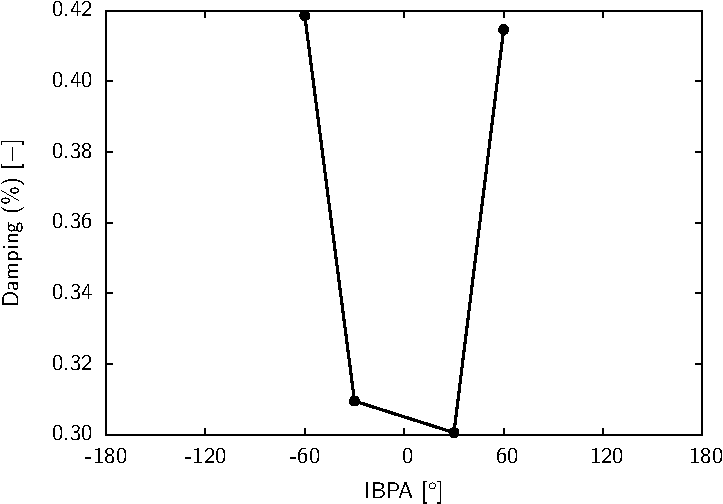
\includegraphics[width=.45\textwidth]{DREAM_HS_DAMPING_MODE_2F.pdf}}
  \subfigure[1T mode]{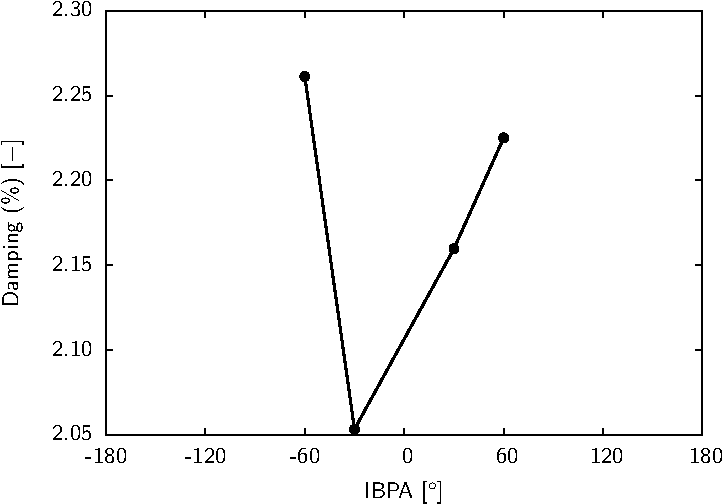
\includegraphics[width=.45\textwidth]{DREAM_HS_DAMPING_MODE_1T.pdf}}
  \caption{High-speed isolated configuration: integrated damping for modes 2F and 1T.}
  \label{fig:dream_hs_ael_damping}
\end{figure}

\subsection{Local excitation}
\label{sub:dream_hs_ael_local_damping}

The local excitation is shown on the pressure side and
the suction side of the front rotor blades in 
Figure~\ref{fig:dream_hs_ael_local_damping}. It is the
local damping given in each cell divided by the 
surface of the cell. It is therefore expressed in
m\textsuperscript{-2}.
\begin{figure}[htp]
 \ra{1.3} \centering
 \begin{tabular}{r|cccc}
   \toprule
   & \multicolumn{4}{c}{
        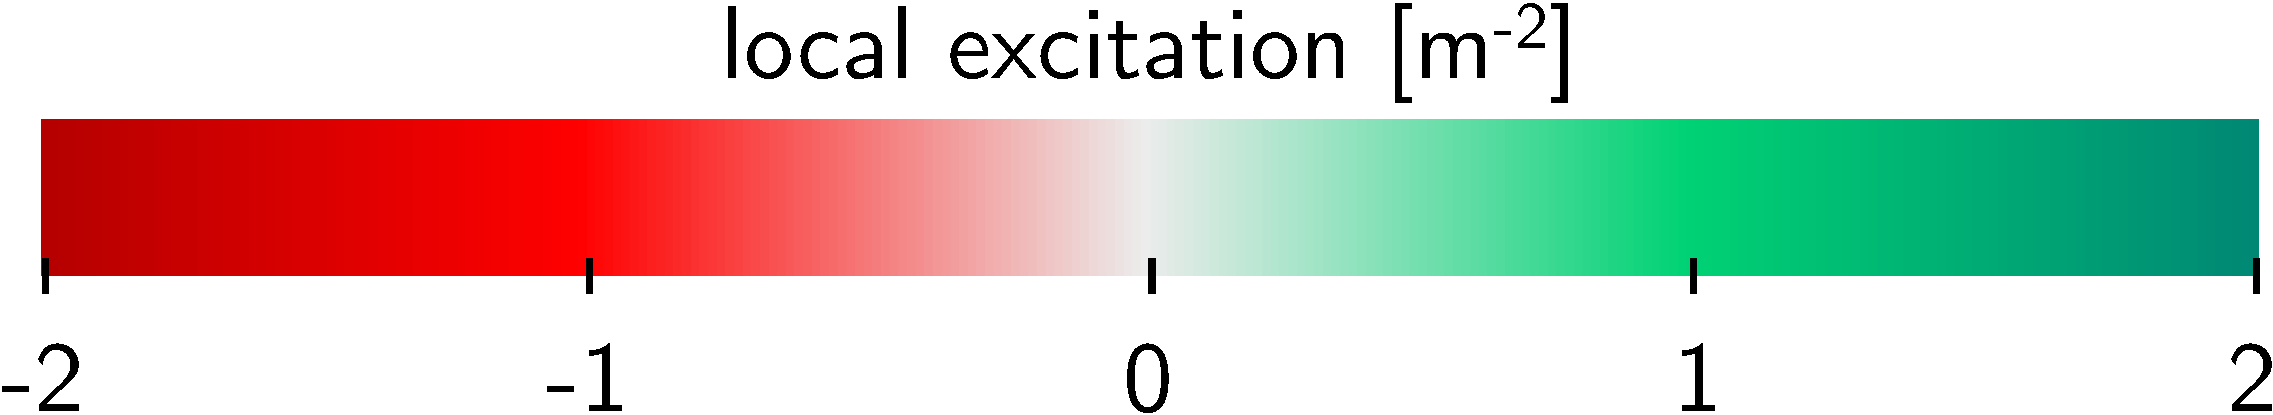
\includegraphics[width=0.22\textwidth]{dream_hs_damping_scale.pdf}} \\
   & \multicolumn{2}{c}{mode 2F} & \multicolumn{2}{c}{mode 1T} \\
   \midrule
   \rotatebox{90}{\quad\quad\quad IBPA $= -60^\circ$} 
   & 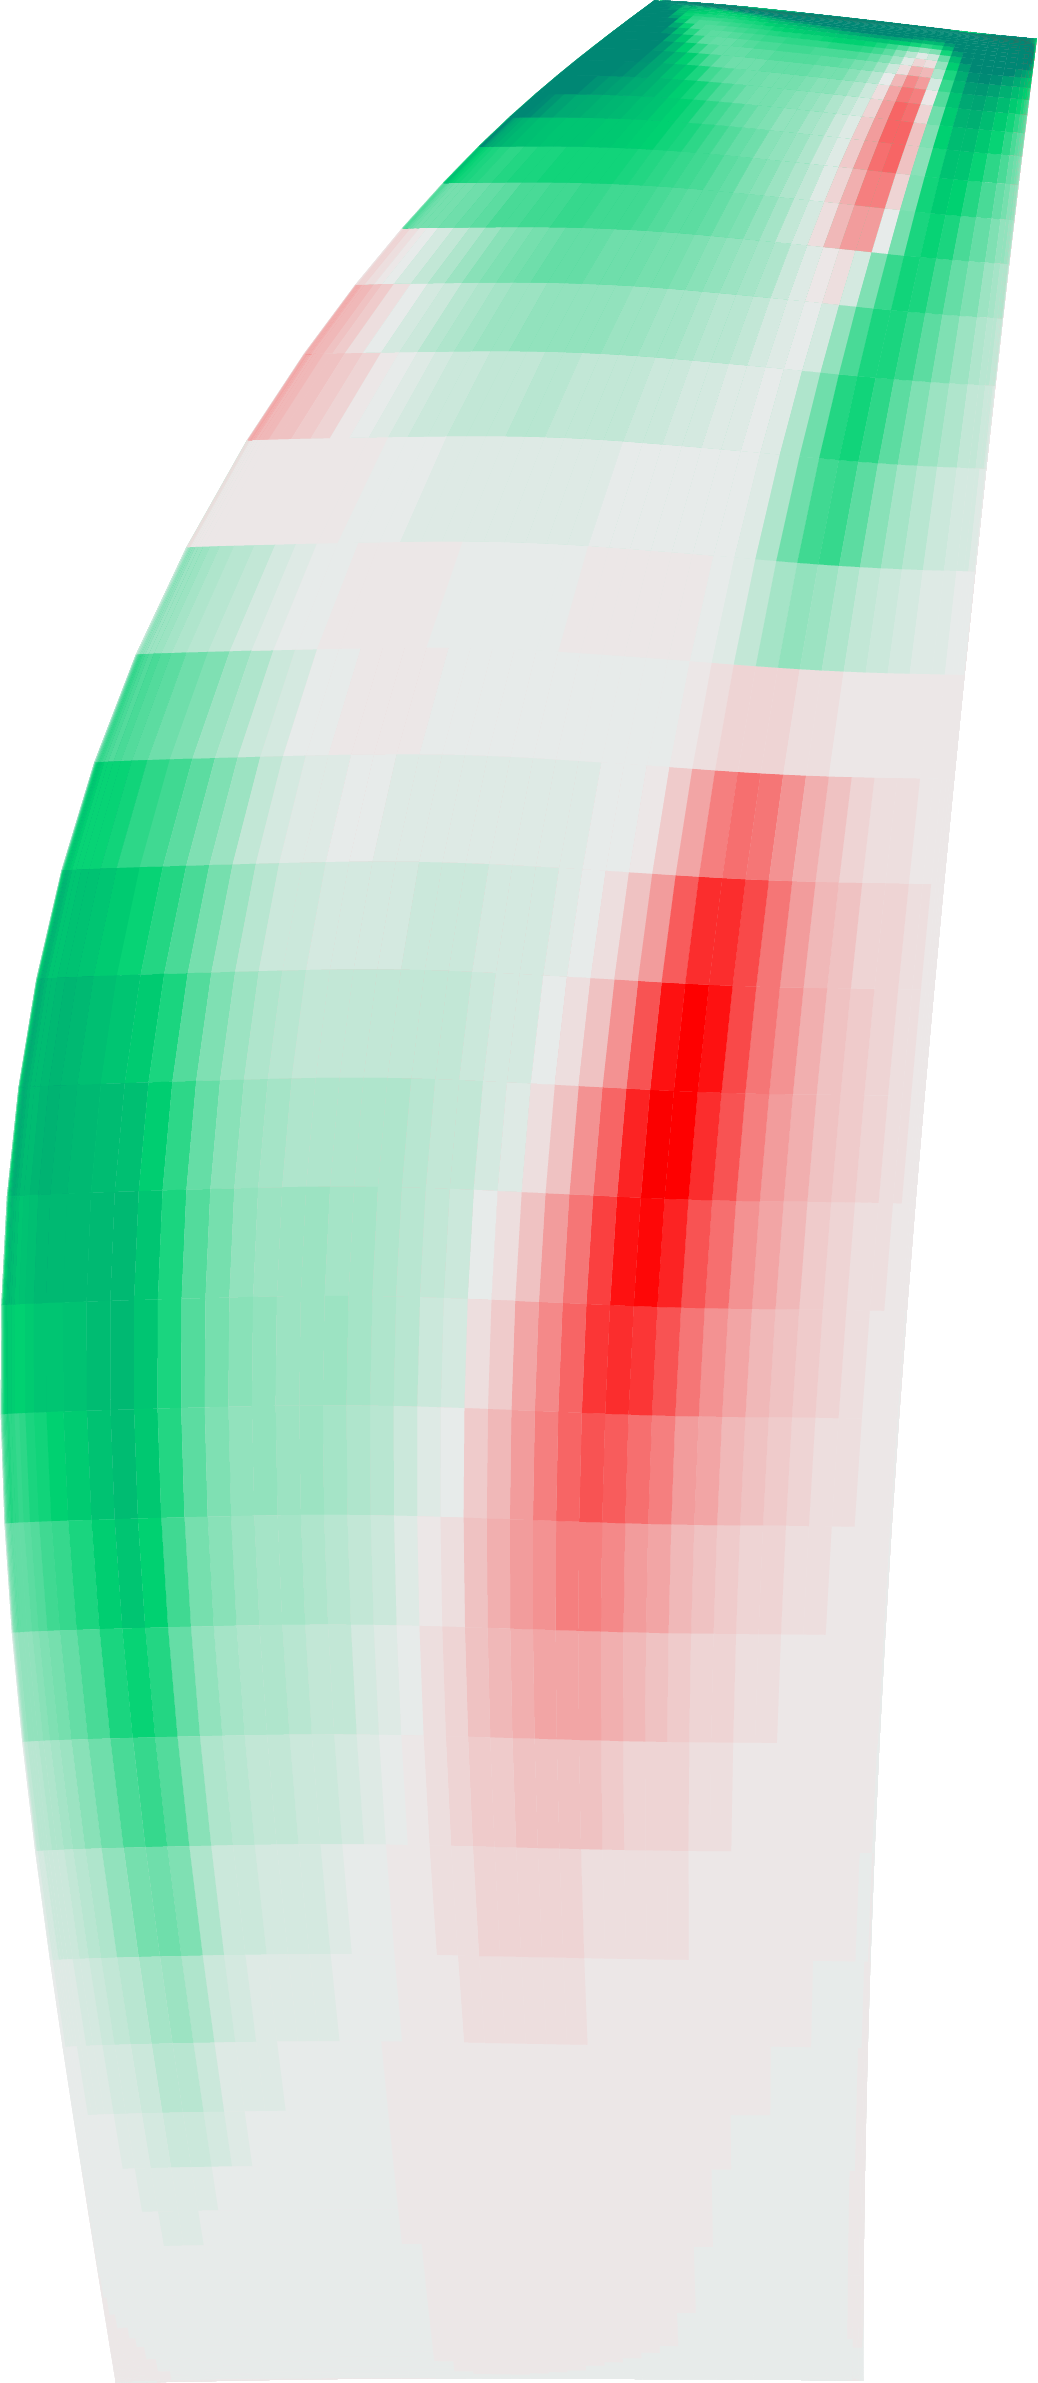
\includegraphics[width=0.12\textwidth]{DREAM_HS_HBT_N5_AEL_H1M2FD-3_roe3_sa_local_damping_SS.png}
   & 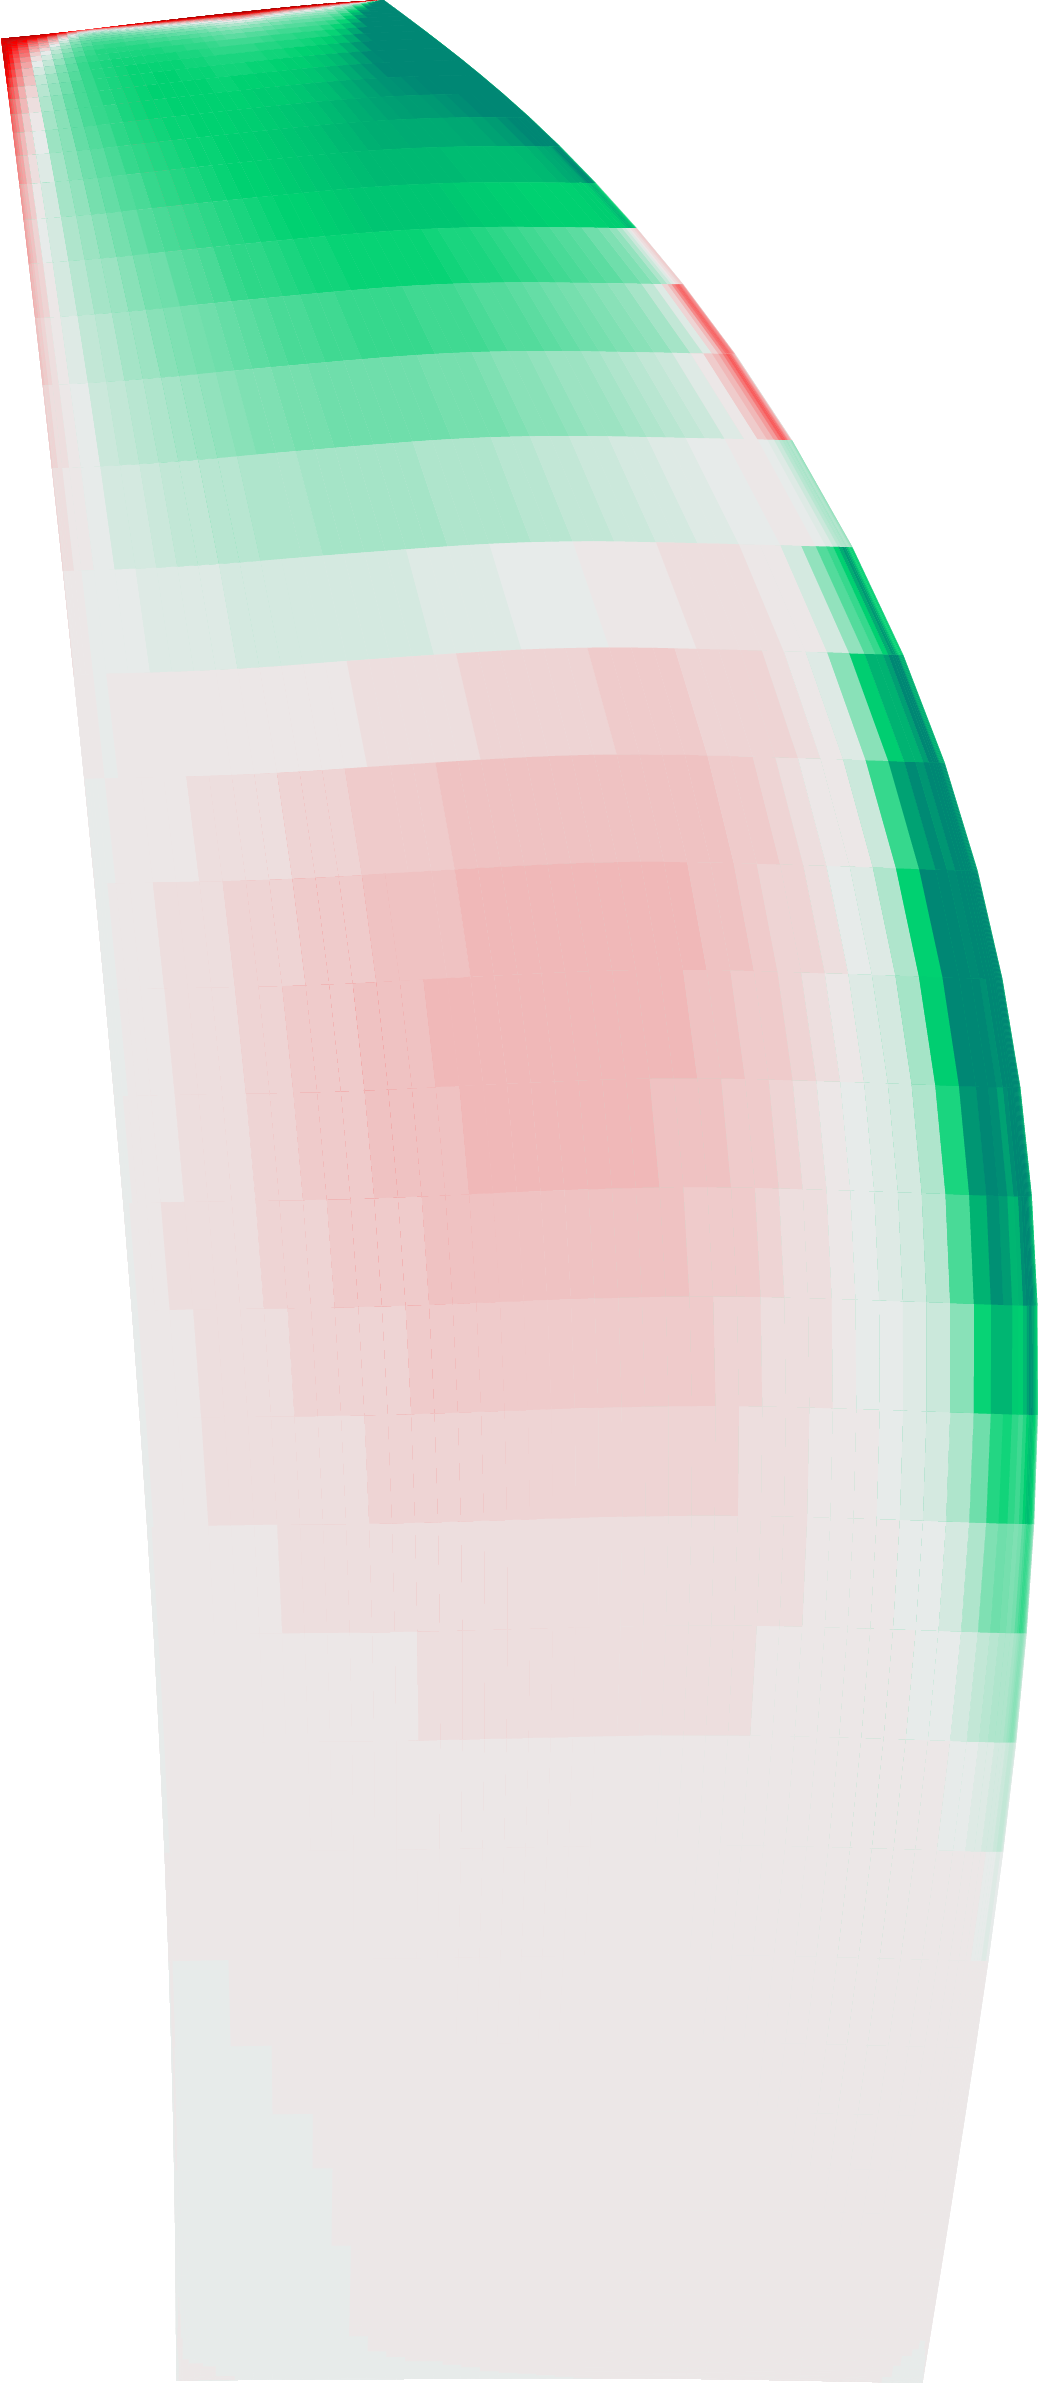
\includegraphics[width=0.12\textwidth]{DREAM_HS_HBT_N5_AEL_H1M2FD-3_roe3_sa_local_damping_PS.png}
   & 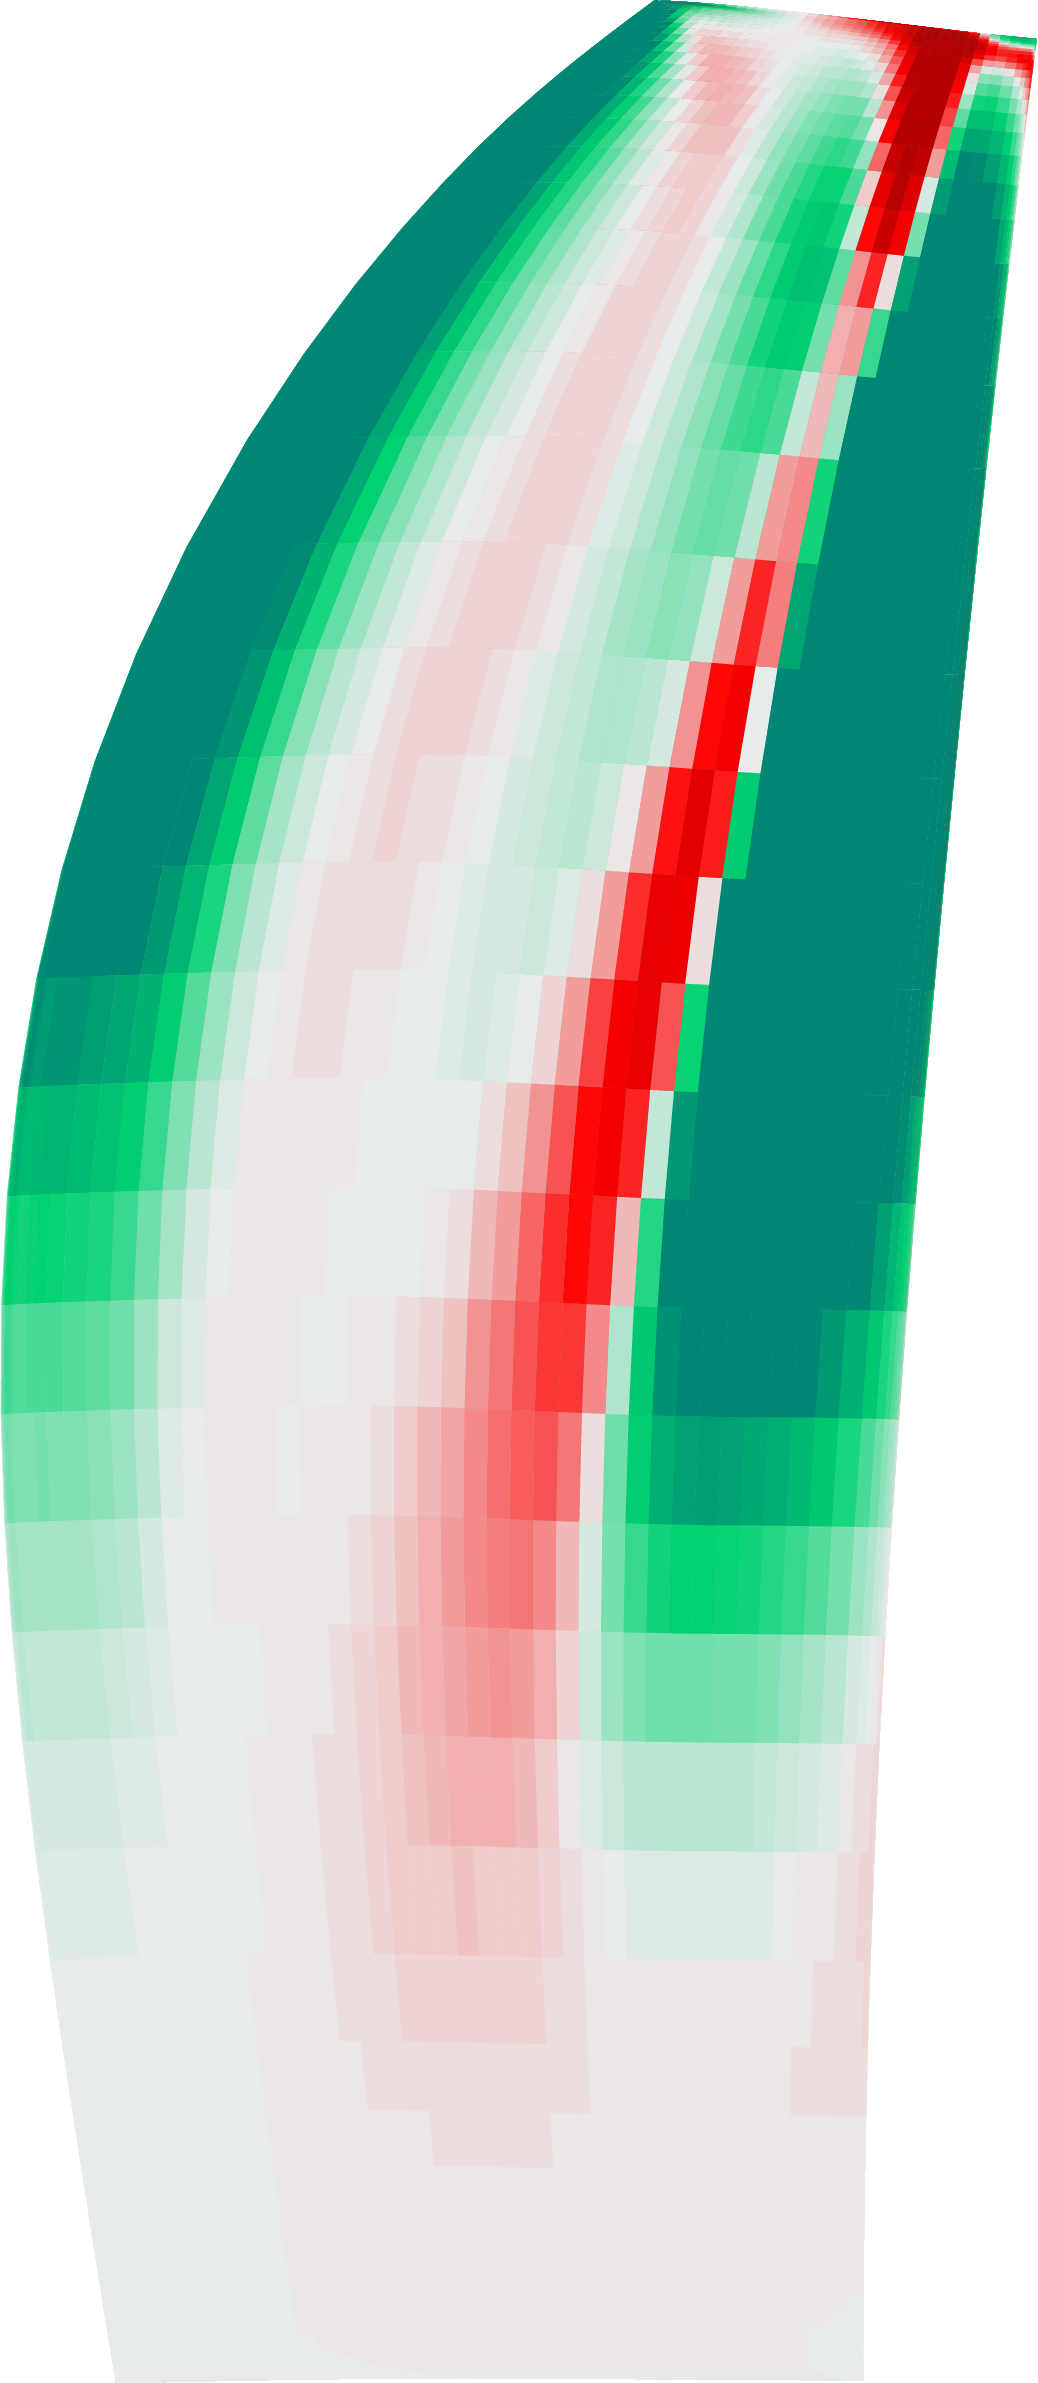
\includegraphics[width=0.12\textwidth]{DREAM_HS_HBT_N5_AEL_H1M1TD-3_roe3_sa_local_damping_SS.png}
   & 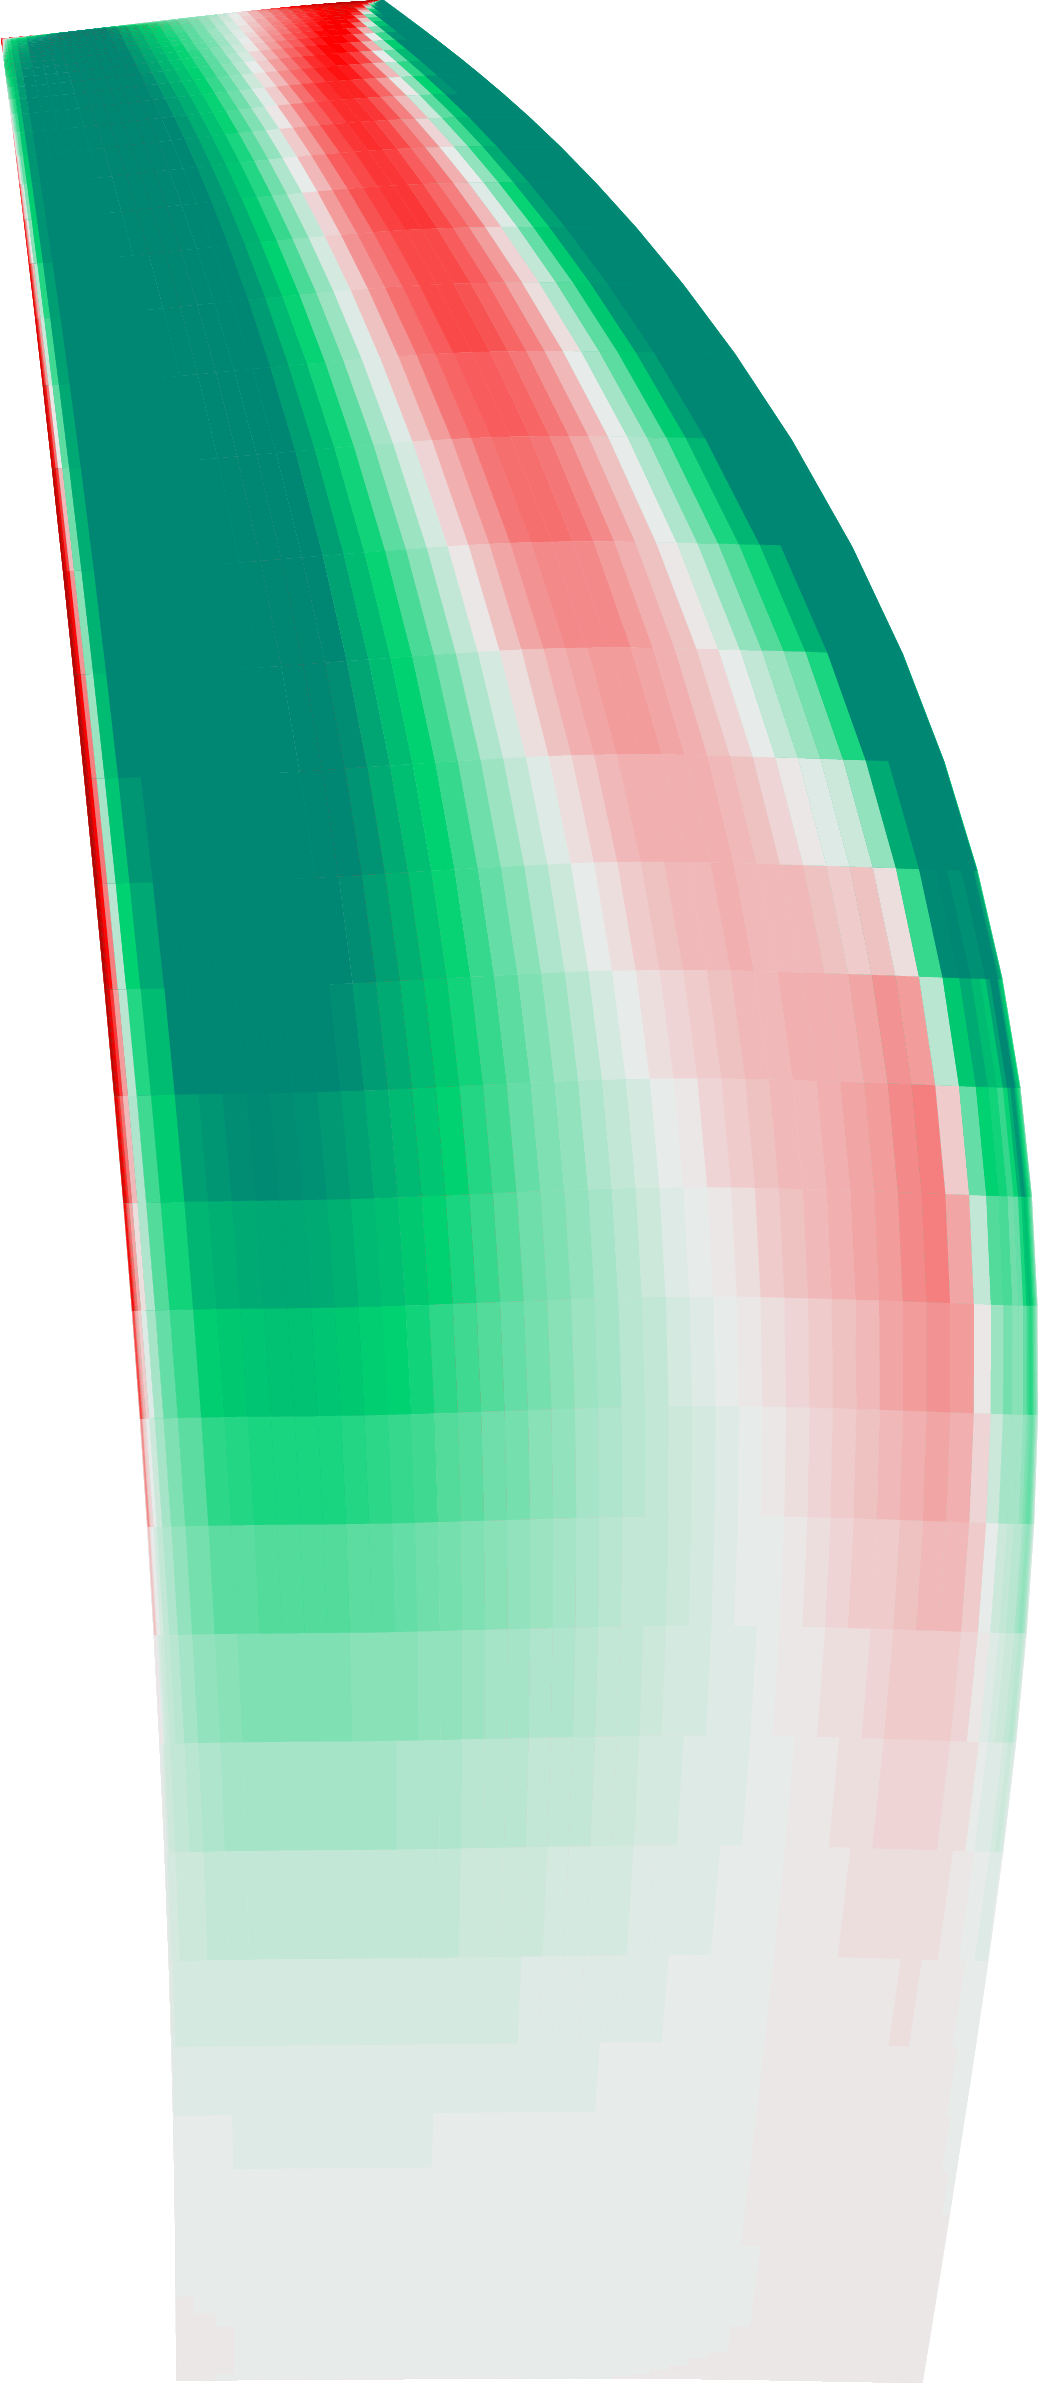
\includegraphics[width=0.12\textwidth]{DREAM_HS_HBT_N5_AEL_H1M1TD-3_roe3_sa_local_damping_PS.png} \\
   \rotatebox{90}{\quad\quad\quad IBPA $= -30^\circ$} 
   & 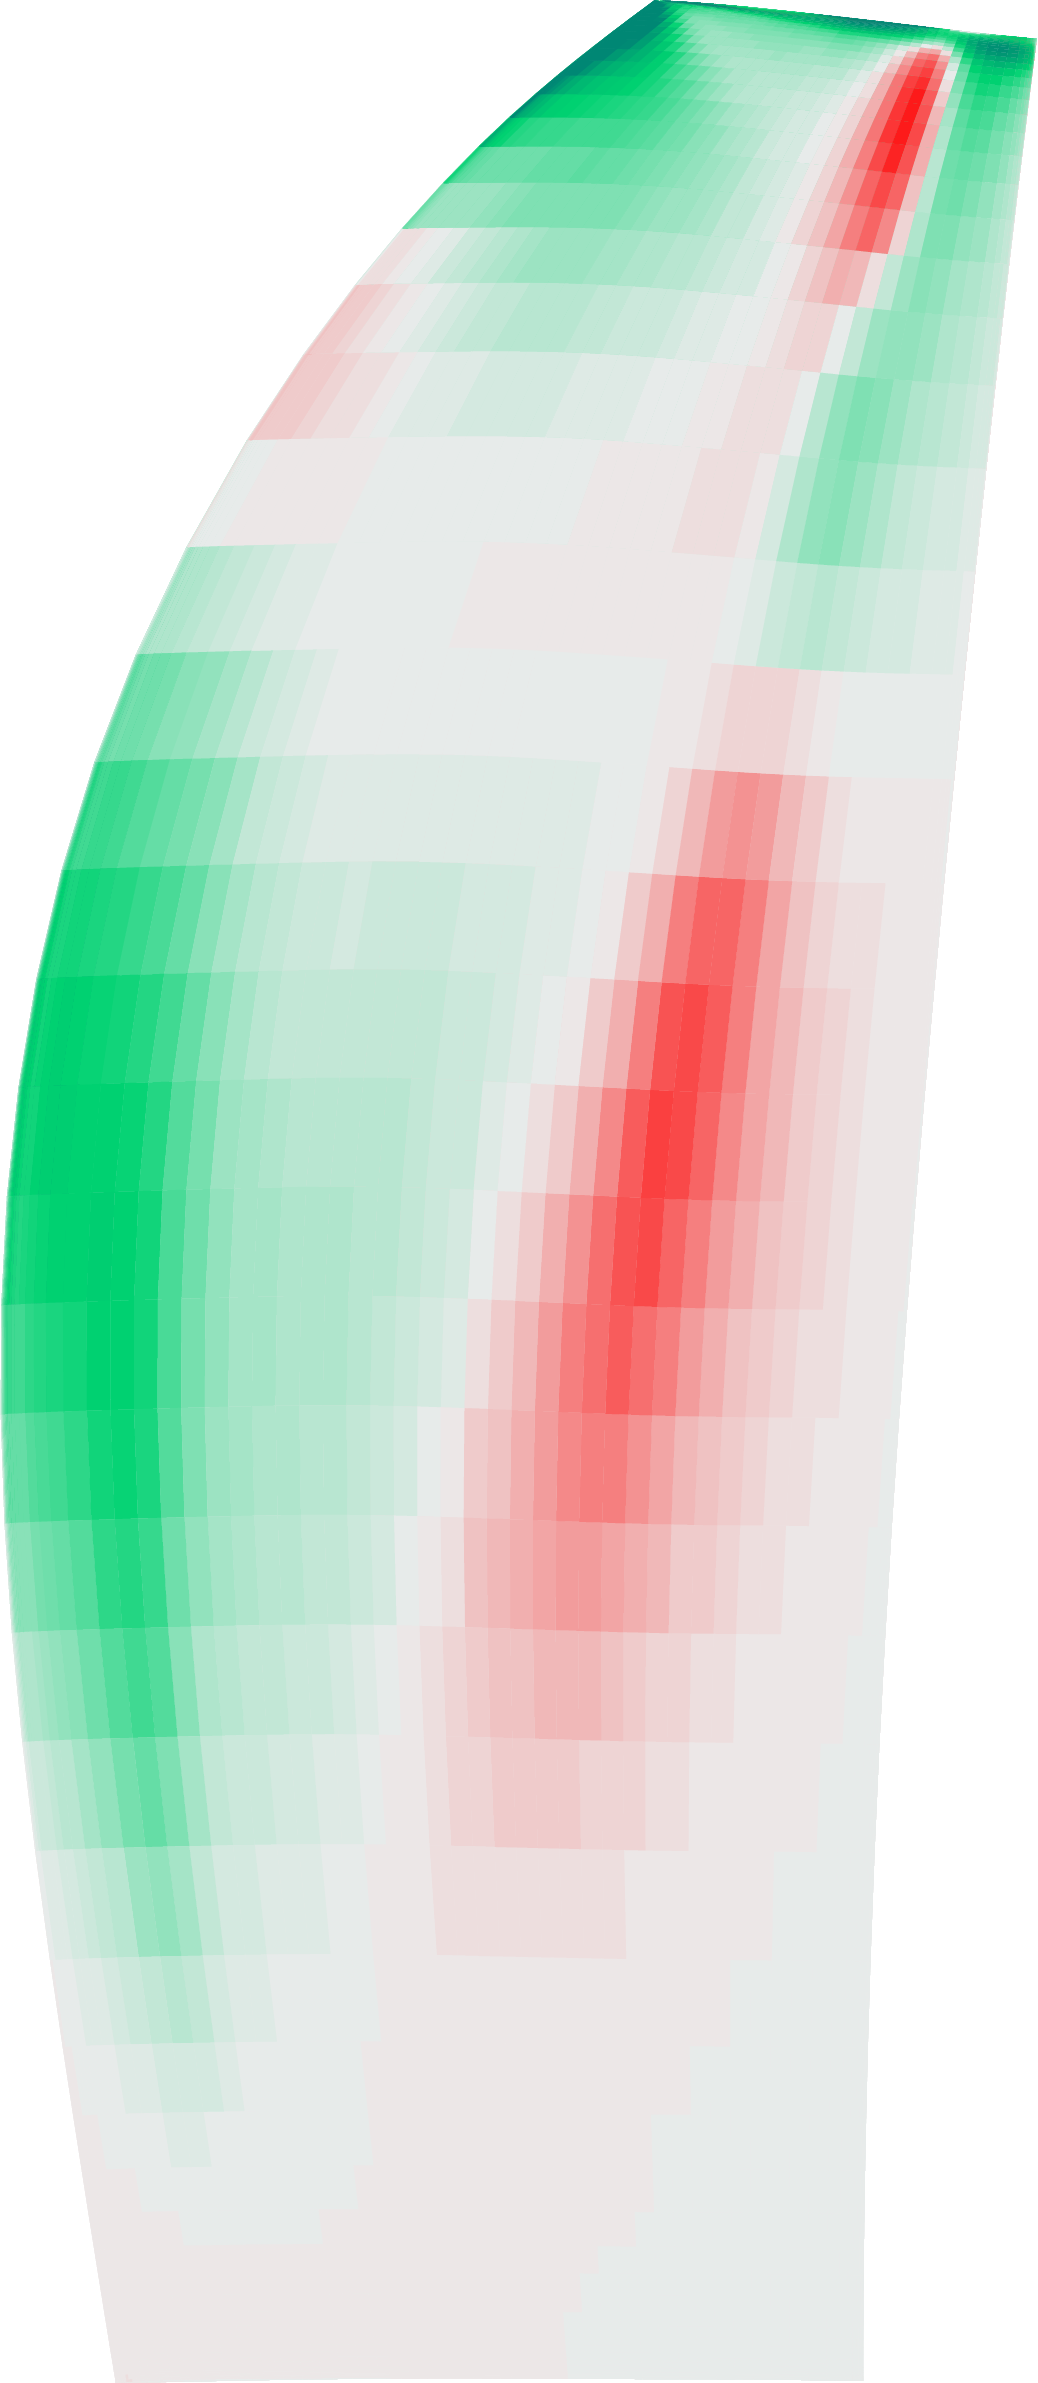
\includegraphics[width=0.12\textwidth]{DREAM_HS_HBT_N5_AEL_H1M2FD-1_roe3_sa_local_damping_SS.png}
   & 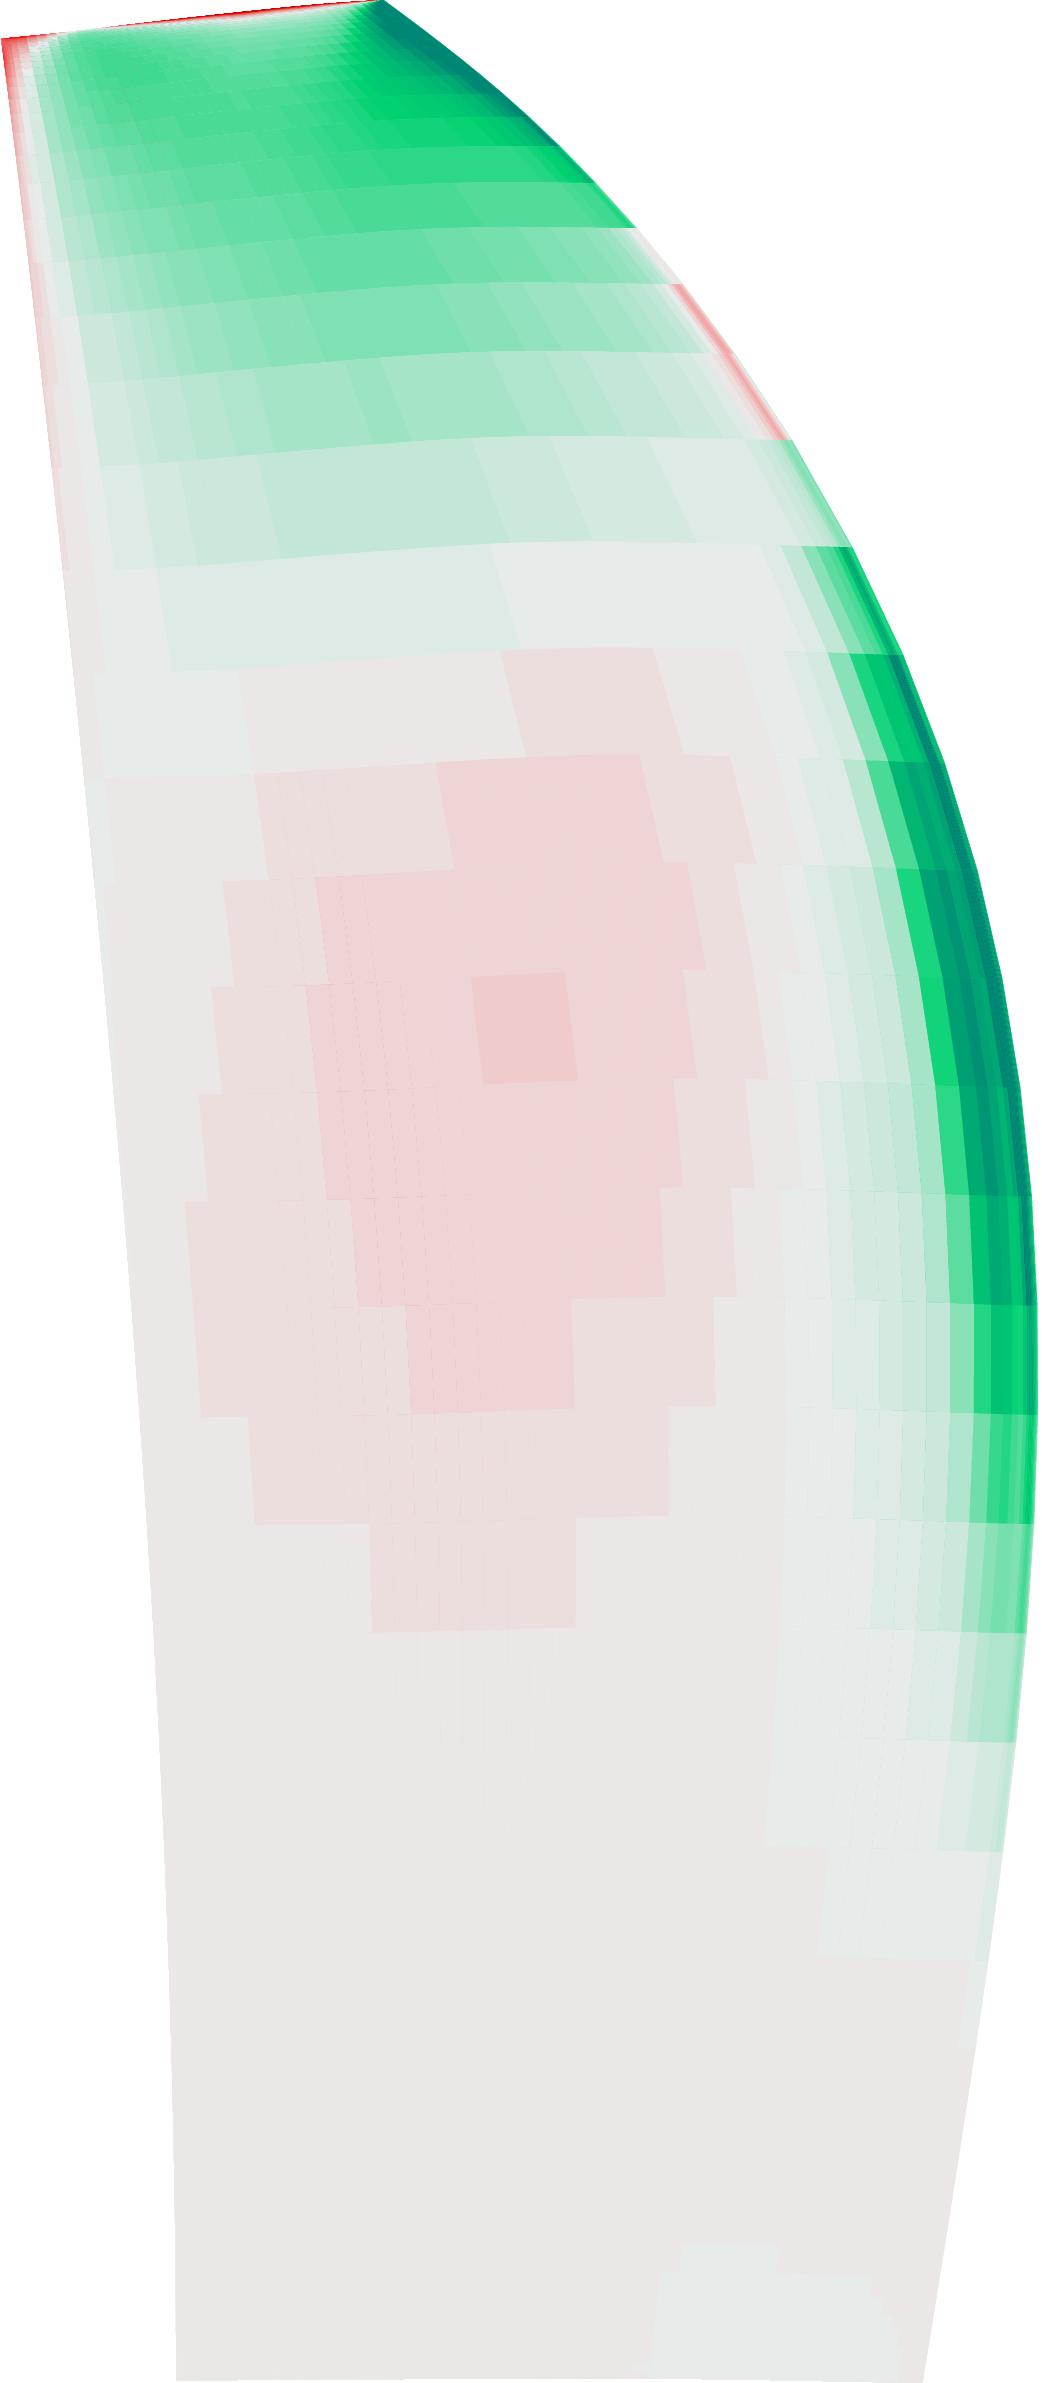
\includegraphics[width=0.12\textwidth]{DREAM_HS_HBT_N5_AEL_H1M2FD-1_roe3_sa_local_damping_PS.png}
   & 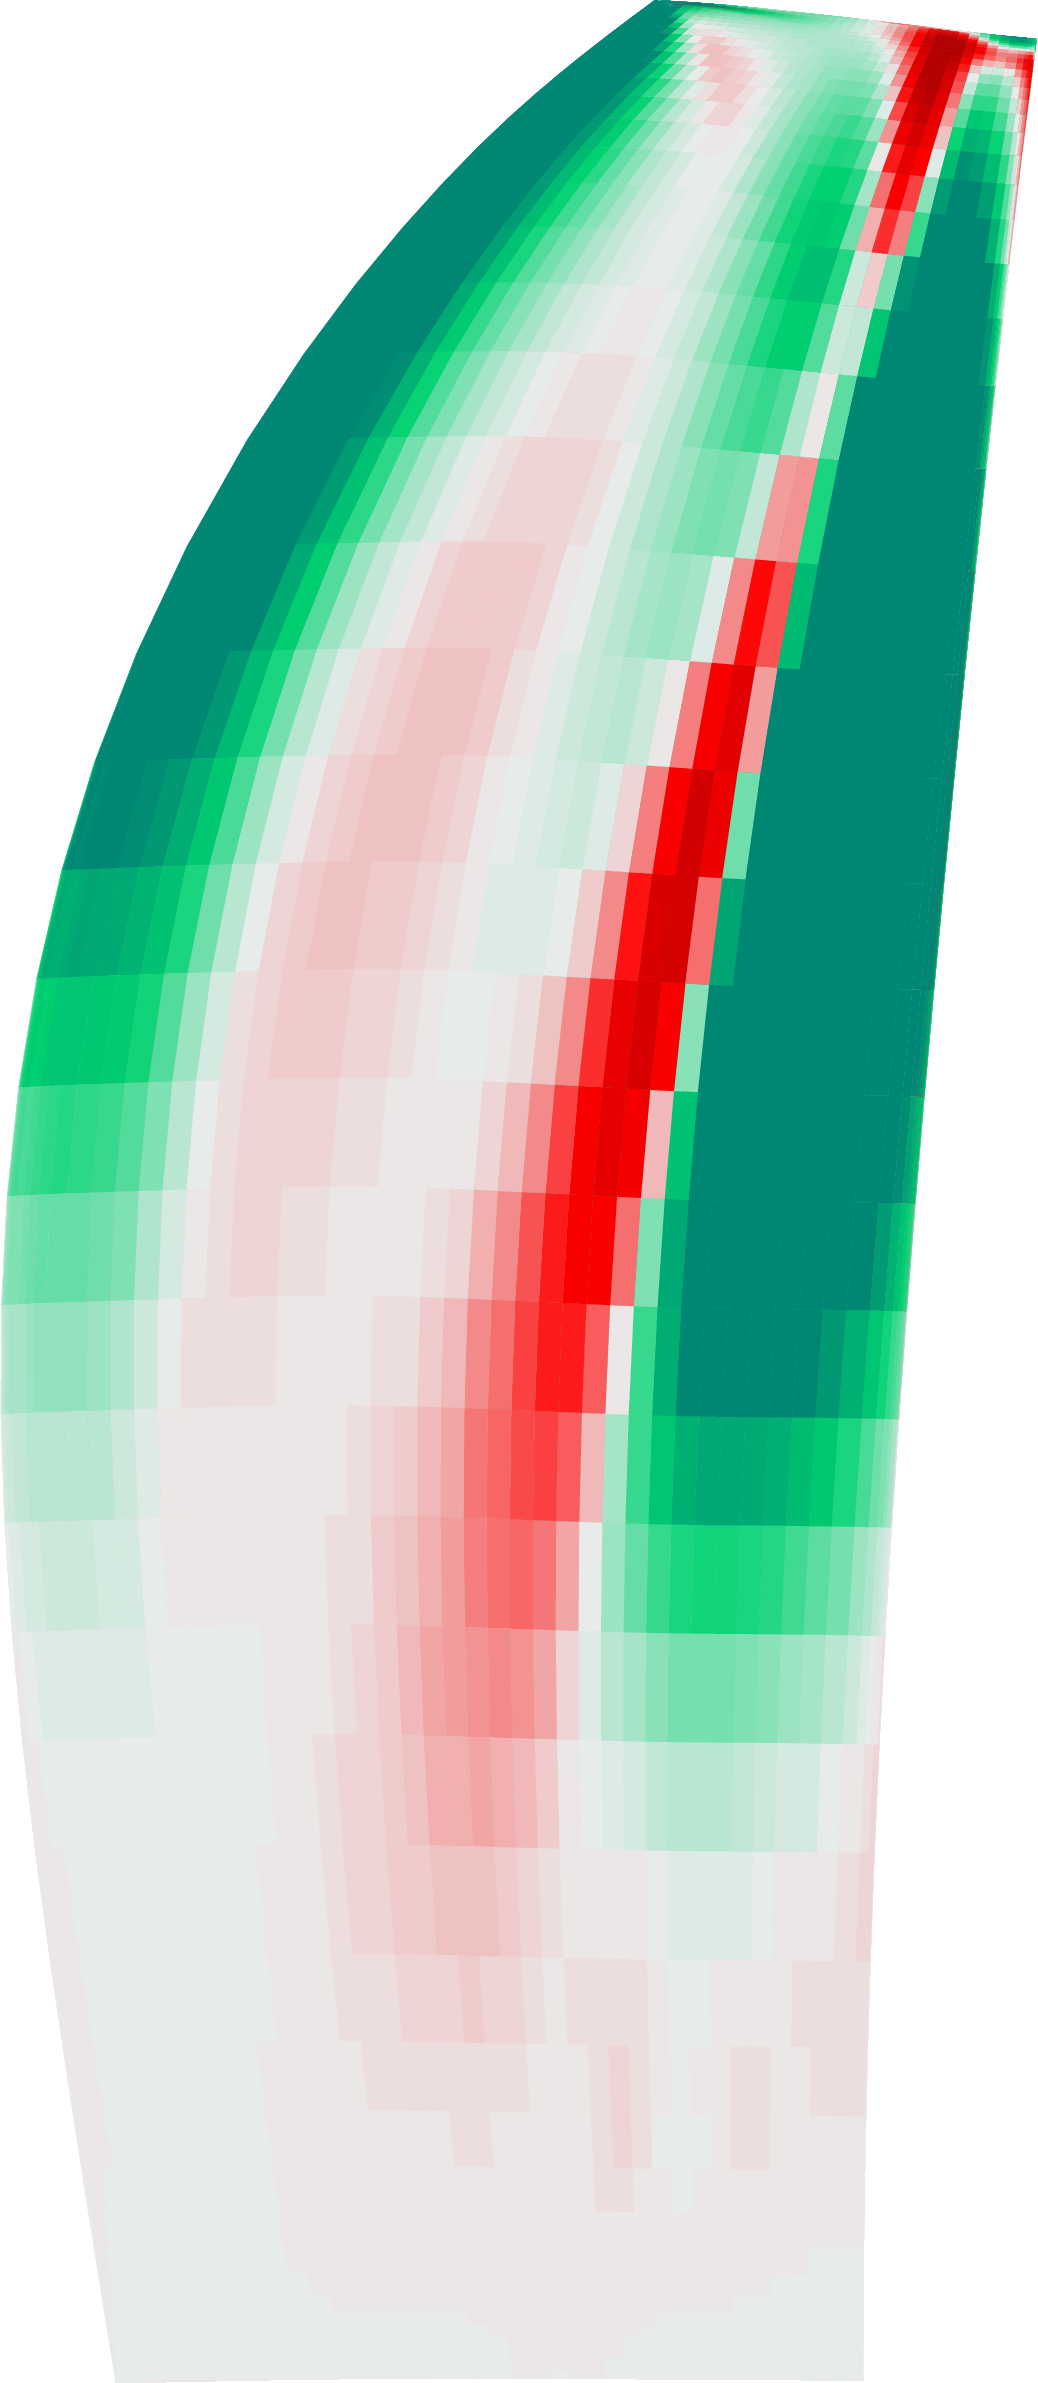
\includegraphics[width=0.12\textwidth]{DREAM_HS_HBT_N5_AEL_H1M1TD-1_roe3_sa_local_damping_SS.png}
   & 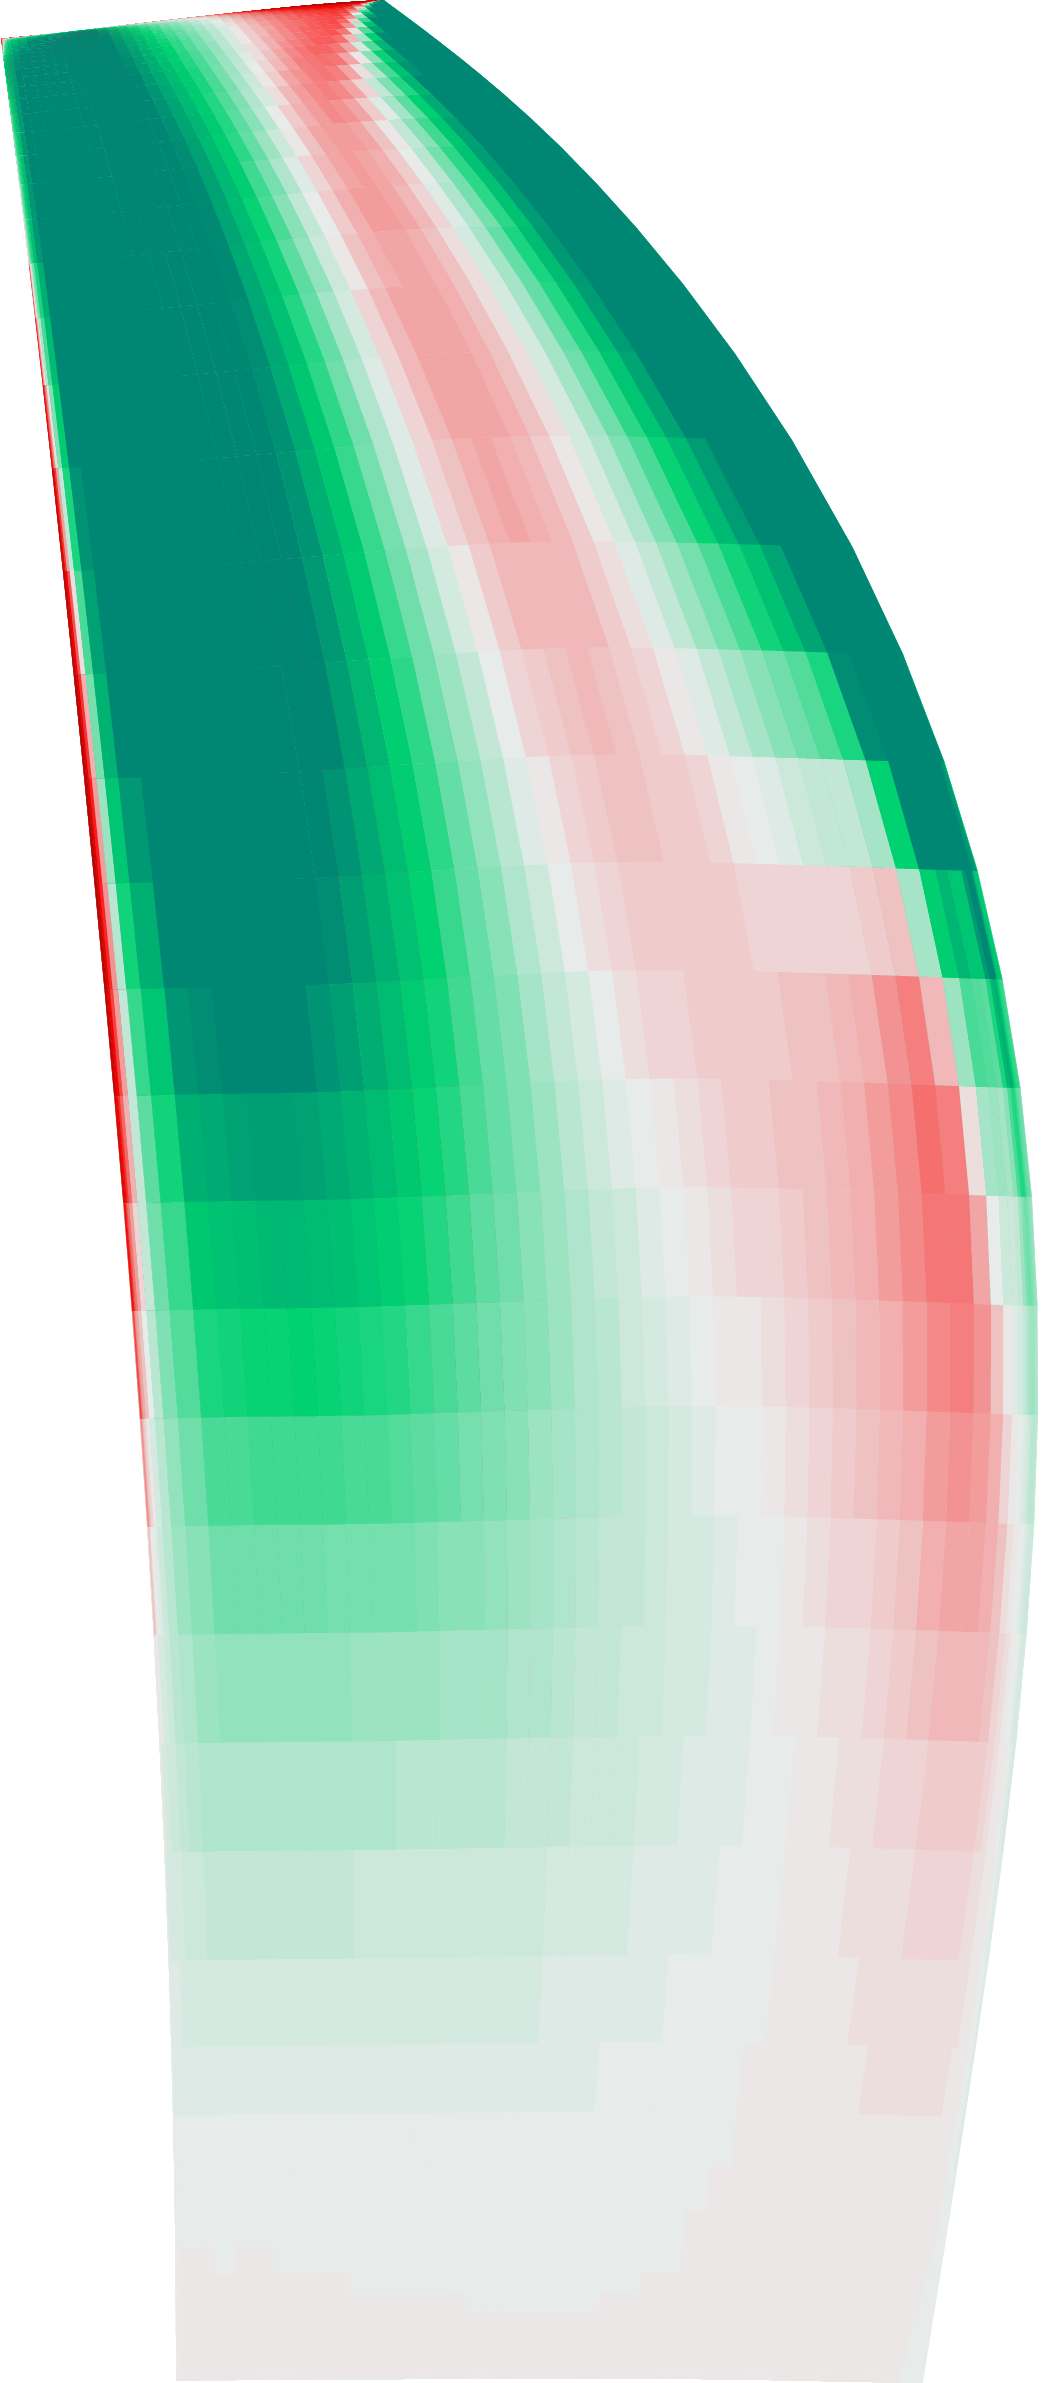
\includegraphics[width=0.12\textwidth]{DREAM_HS_HBT_N5_AEL_H1M1TD-1_roe3_sa_local_damping_PS.png} \\
   \rotatebox{90}{\quad\quad\quad IBPA $= 30^\circ$} 
   & 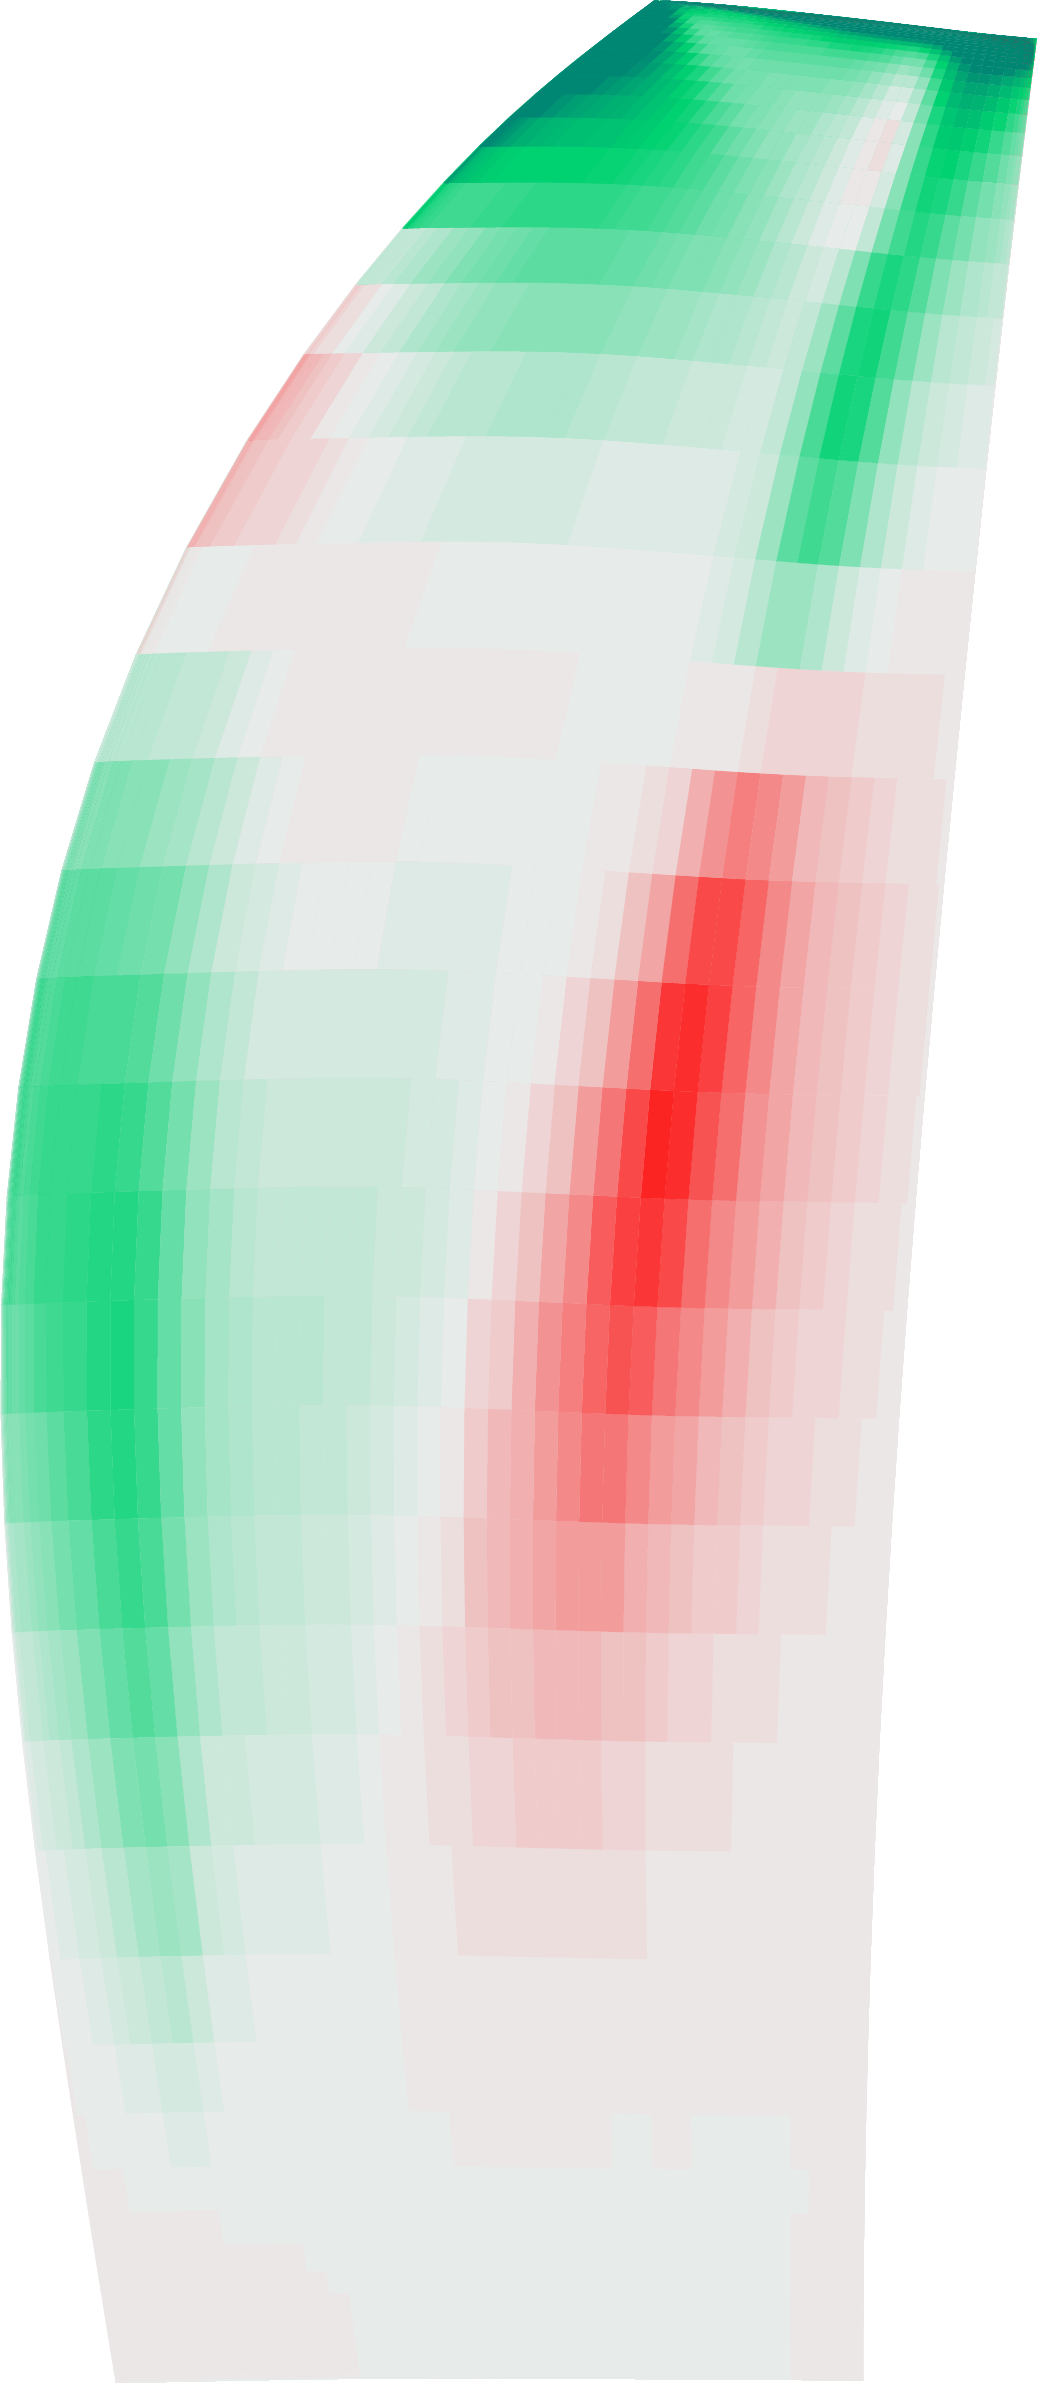
\includegraphics[width=0.12\textwidth]{DREAM_HS_HBT_N5_AEL_H1M2FD1_roe3_sa_local_damping_SS.png}
   & 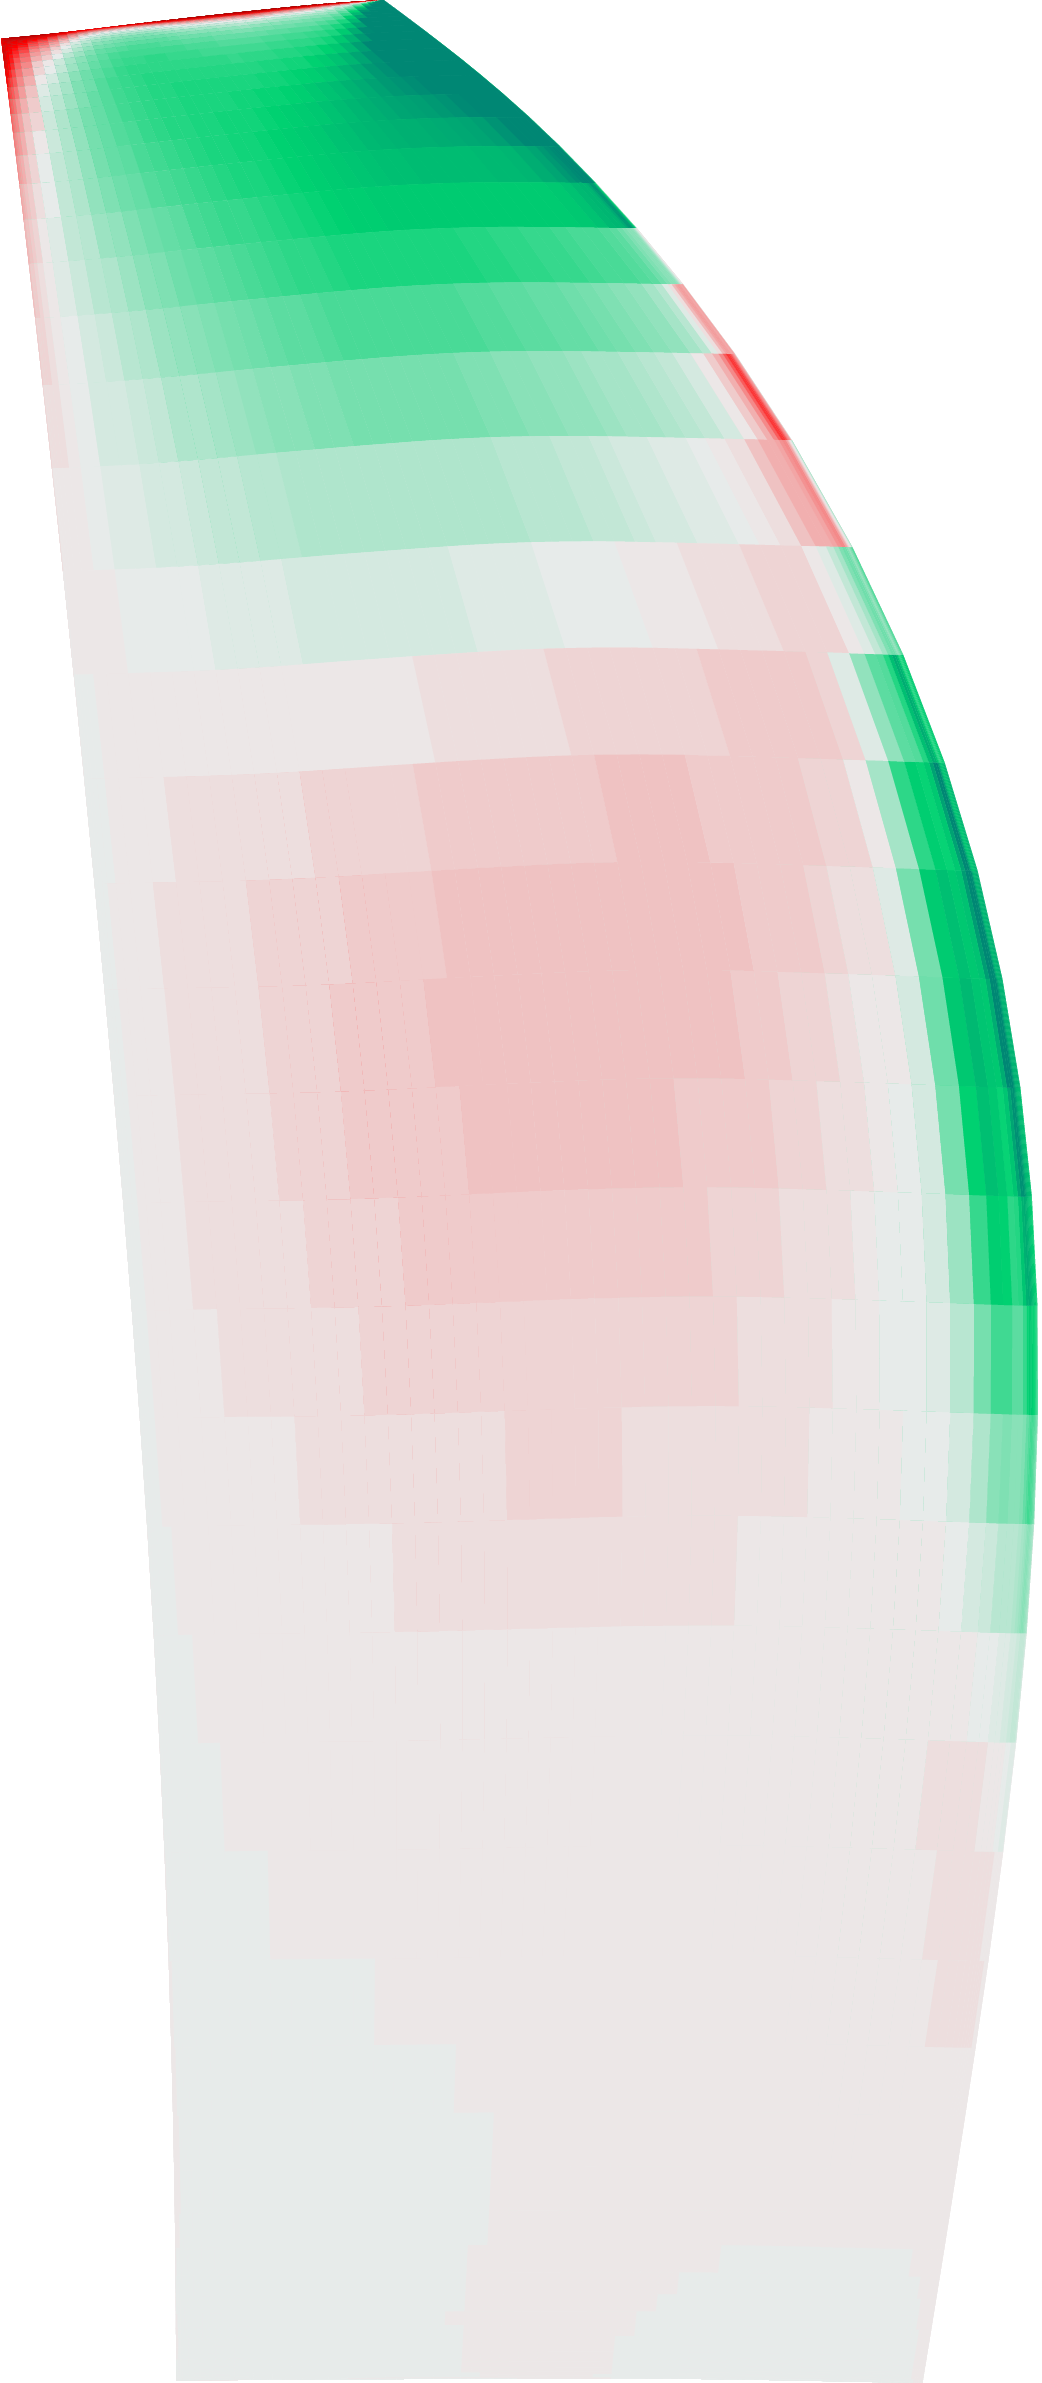
\includegraphics[width=0.12\textwidth]{DREAM_HS_HBT_N5_AEL_H1M2FD1_roe3_sa_local_damping_PS.png}
   & 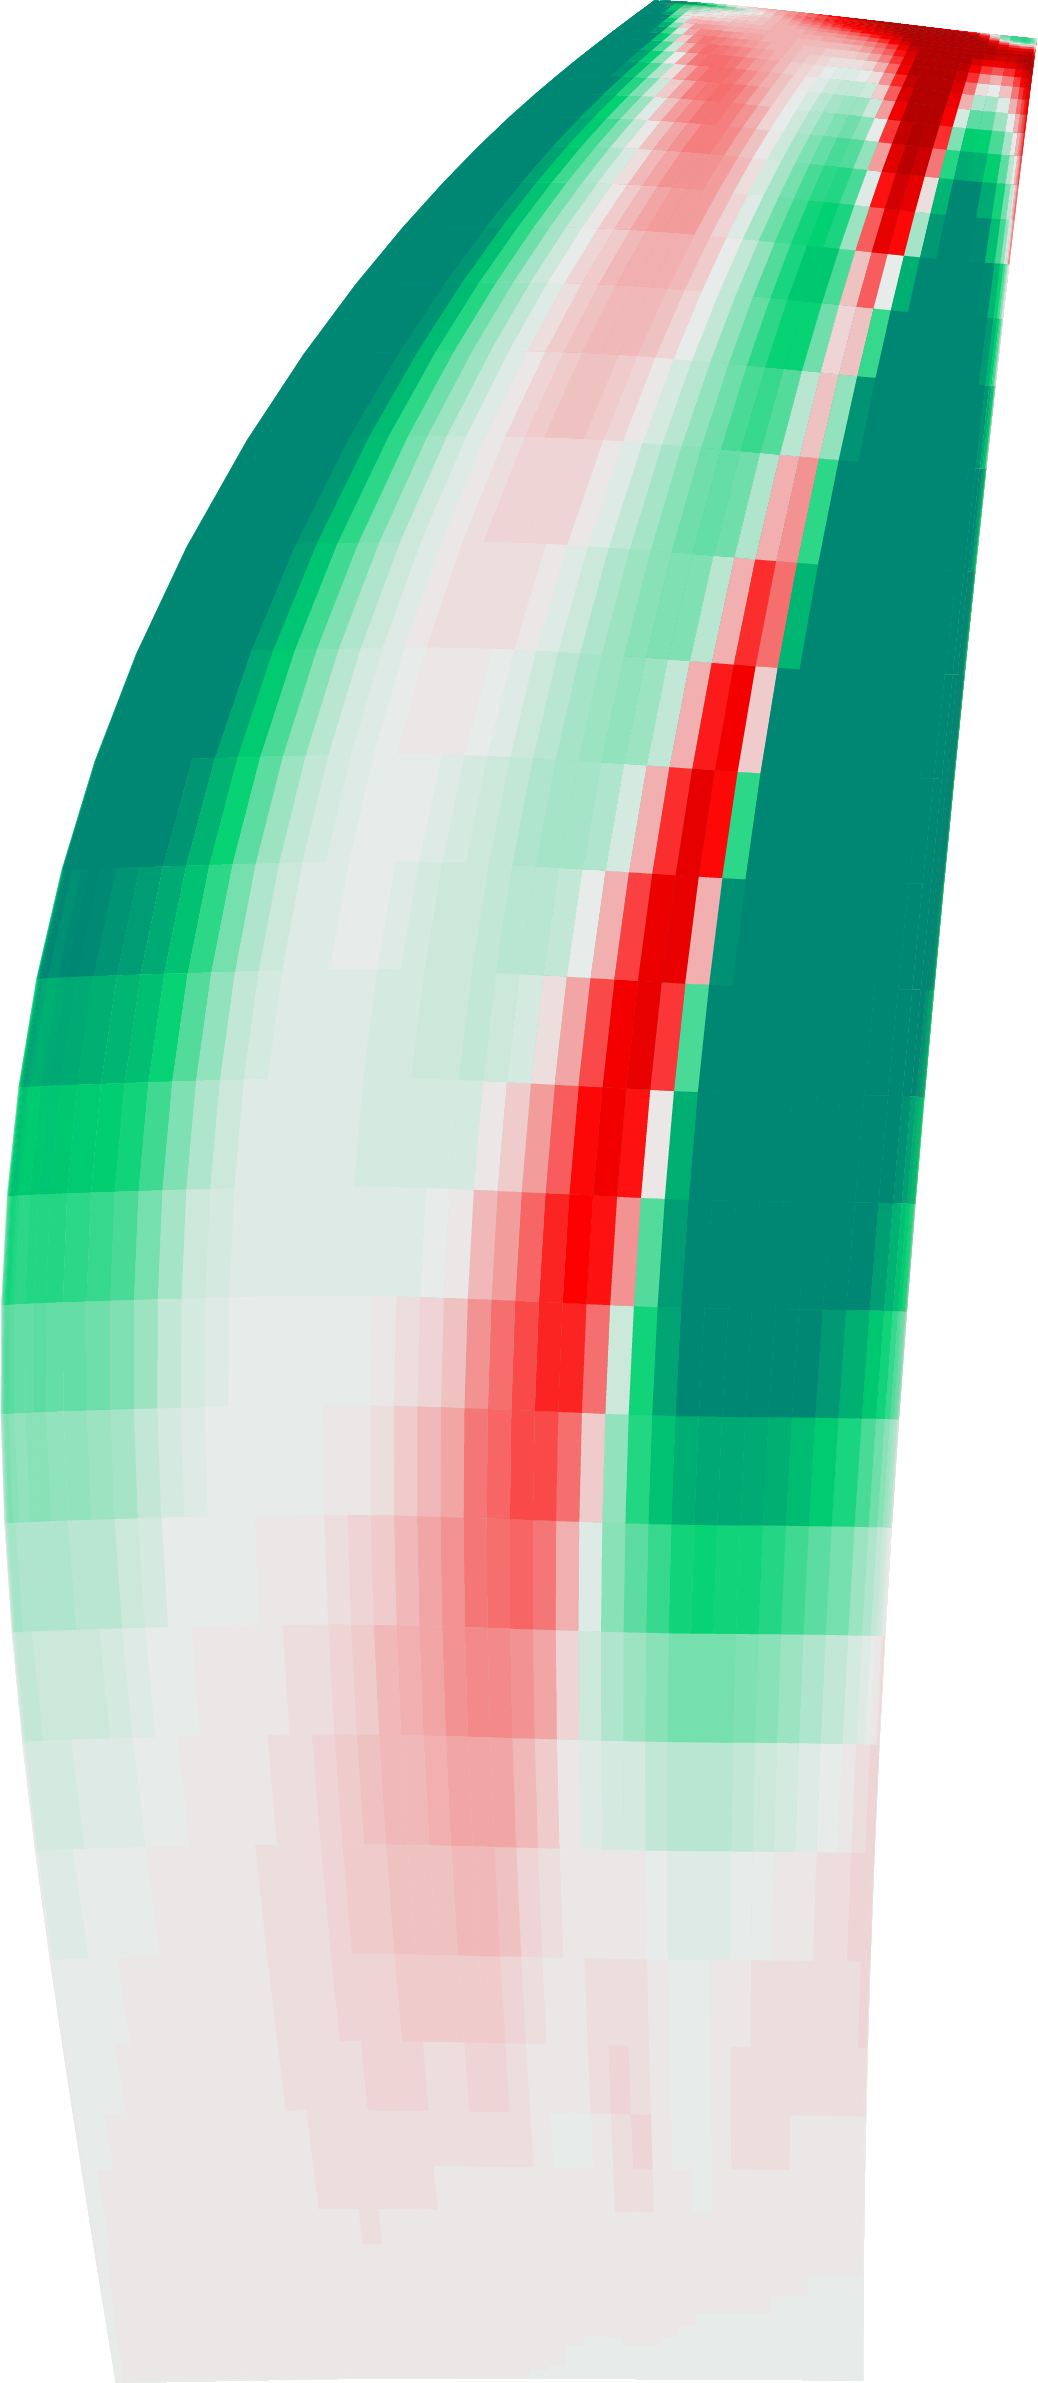
\includegraphics[width=0.12\textwidth]{DREAM_HS_HBT_N5_AEL_H1M1TD1_roe3_sa_local_damping_SS.png}
   & 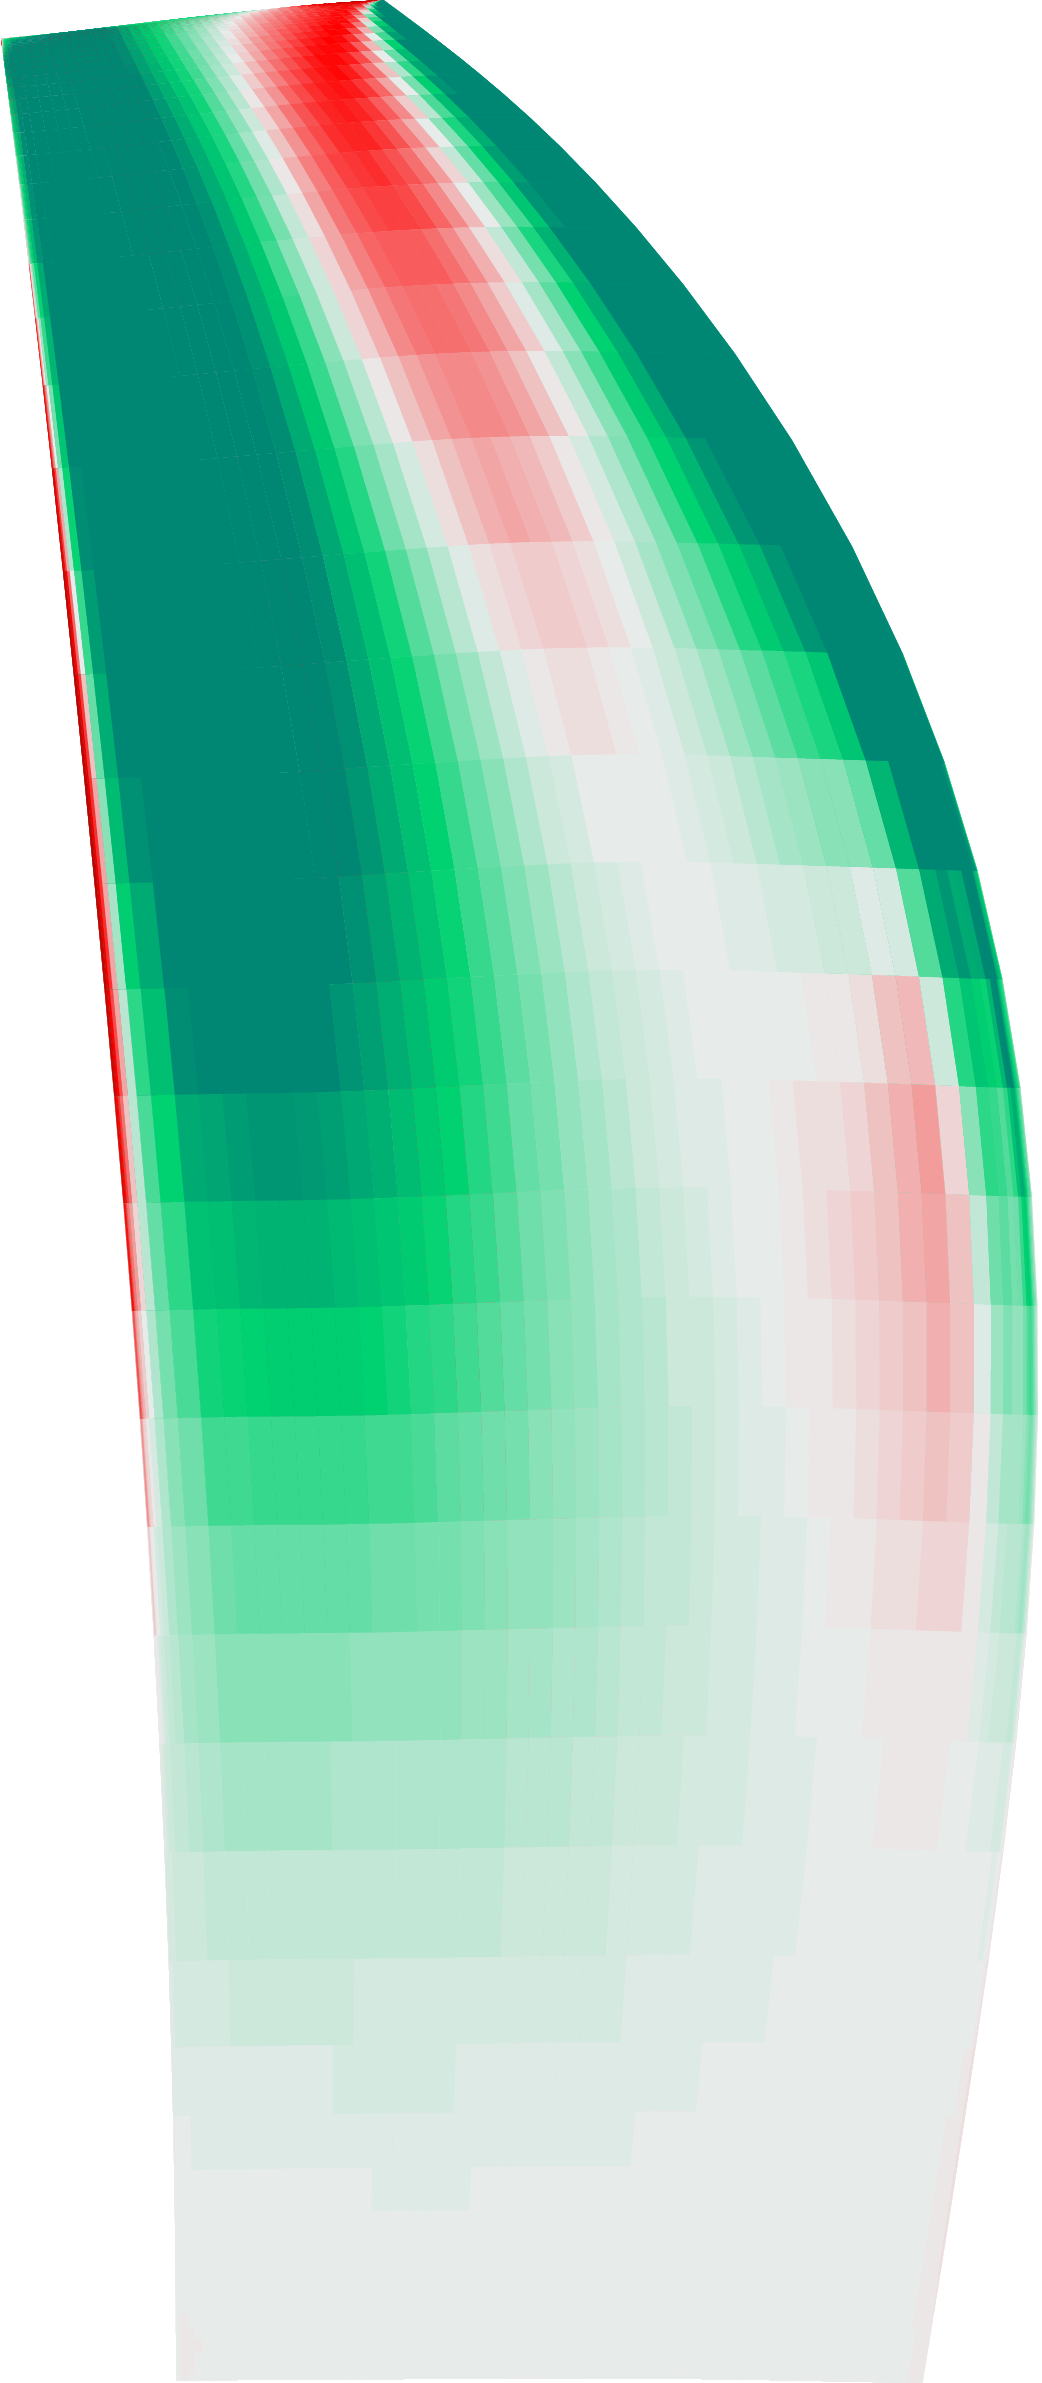
\includegraphics[width=0.12\textwidth]{DREAM_HS_HBT_N5_AEL_H1M1TD1_roe3_sa_local_damping_PS.png} \\
   \rotatebox{90}{\quad\quad\quad IBPA $= 60^\circ$} 
   & 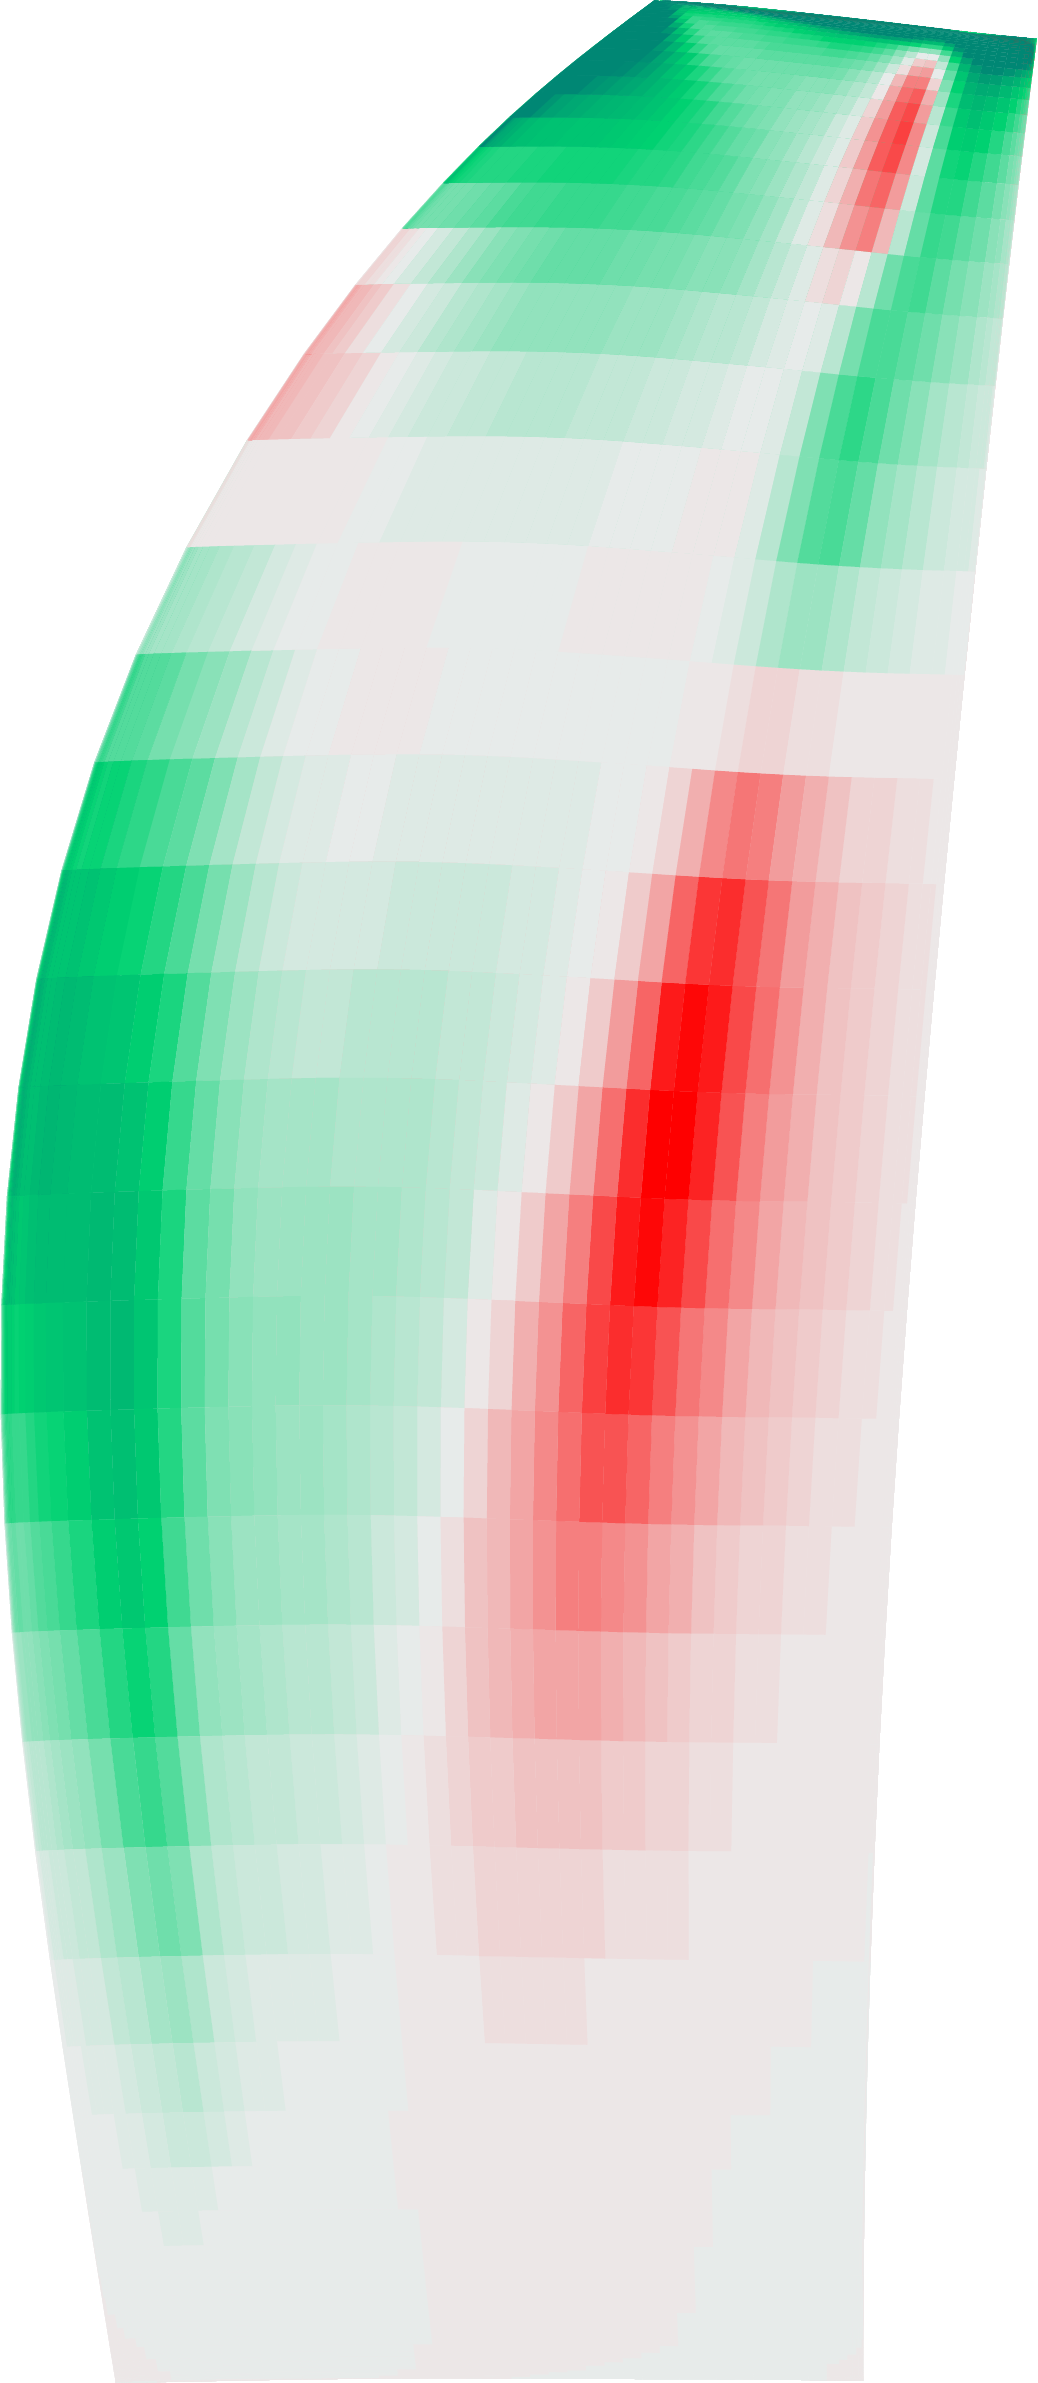
\includegraphics[width=0.12\textwidth]{DREAM_HS_HBT_N5_AEL_H1M2FD3_roe3_sa_local_damping_SS.png}
   & 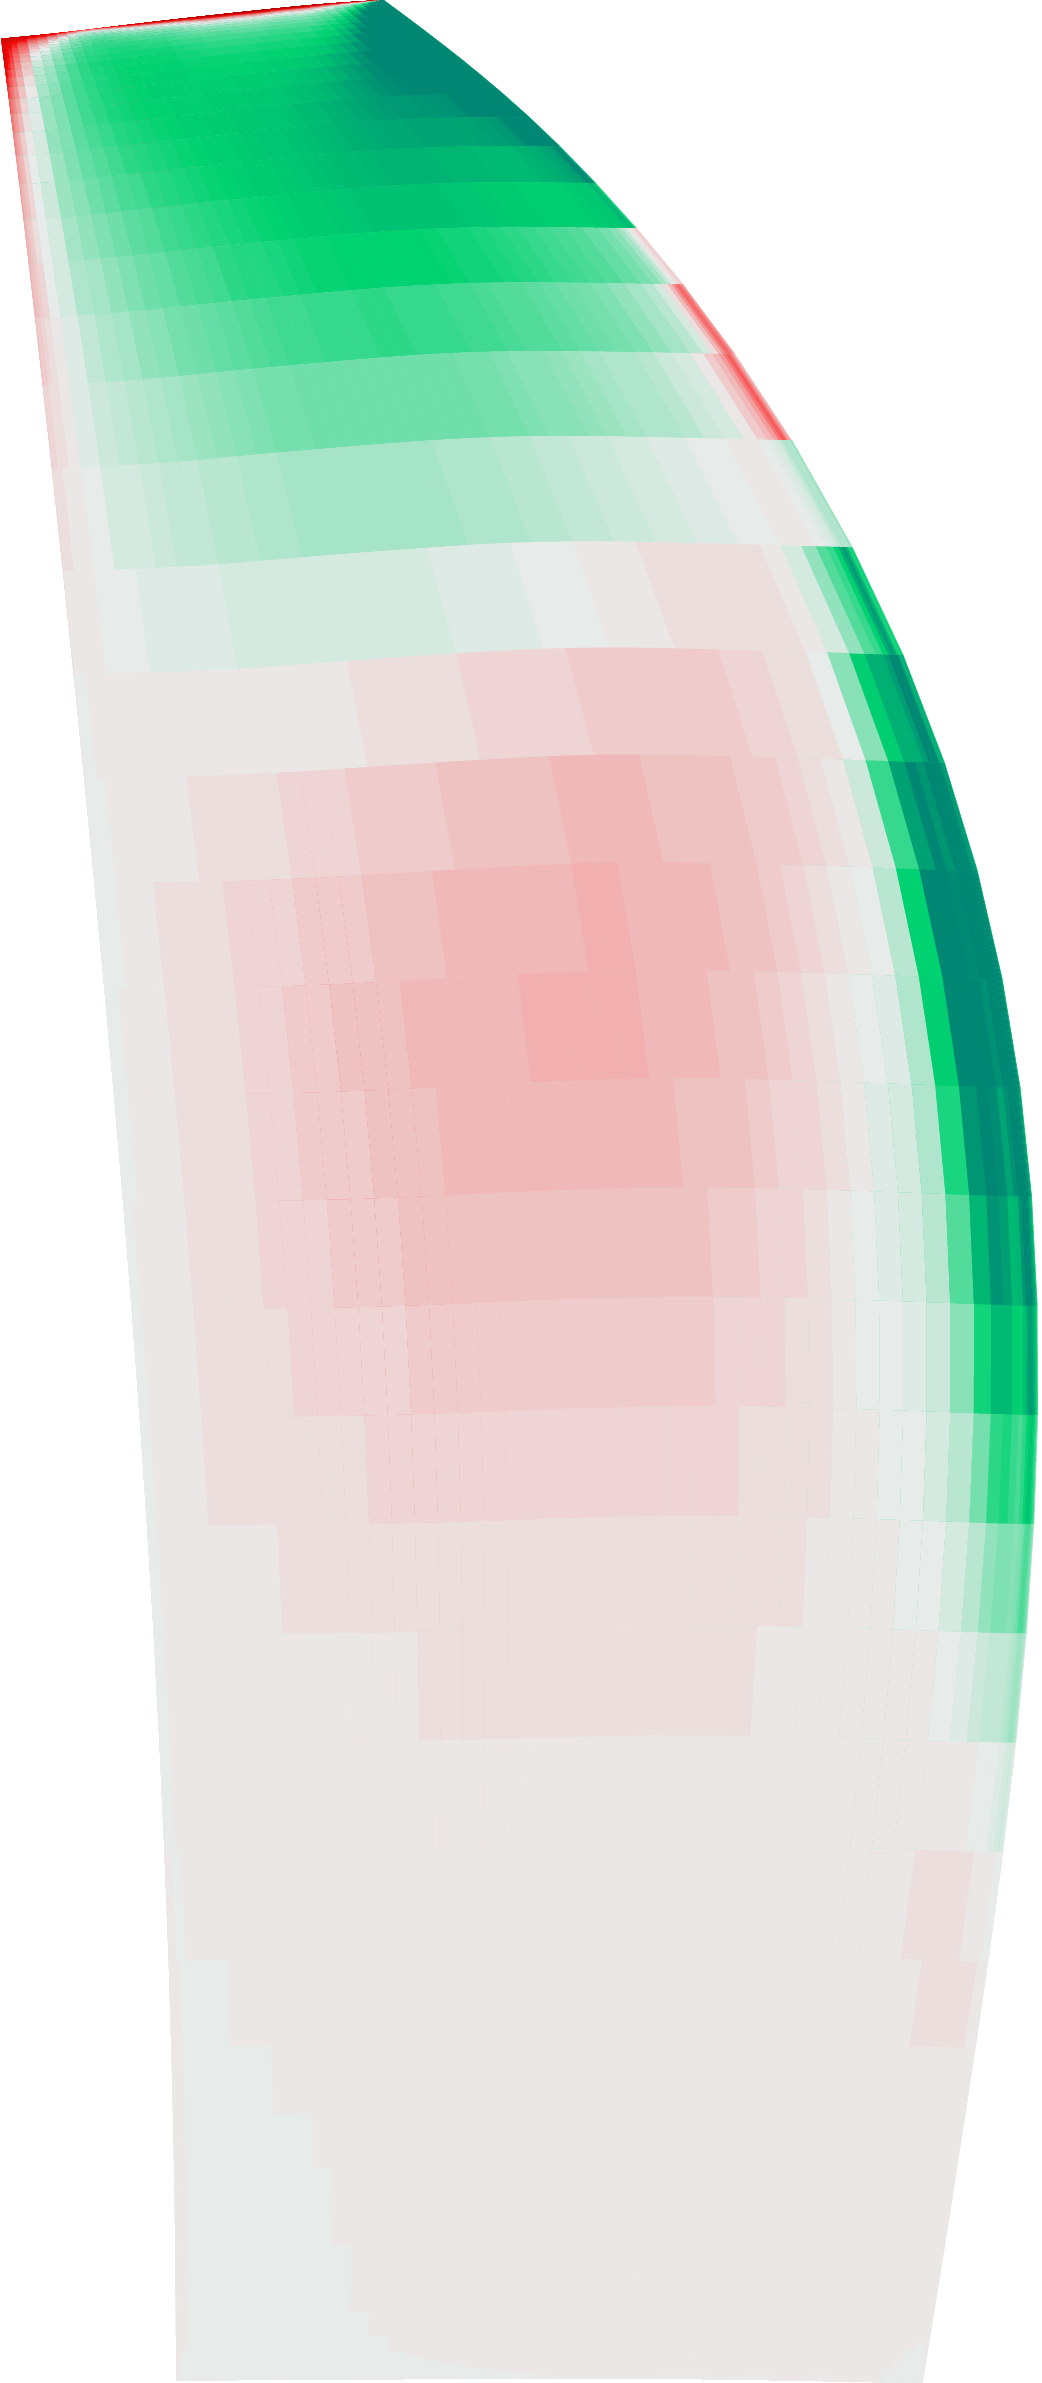
\includegraphics[width=0.12\textwidth]{DREAM_HS_HBT_N5_AEL_H1M2FD3_roe3_sa_local_damping_PS.png}
   & 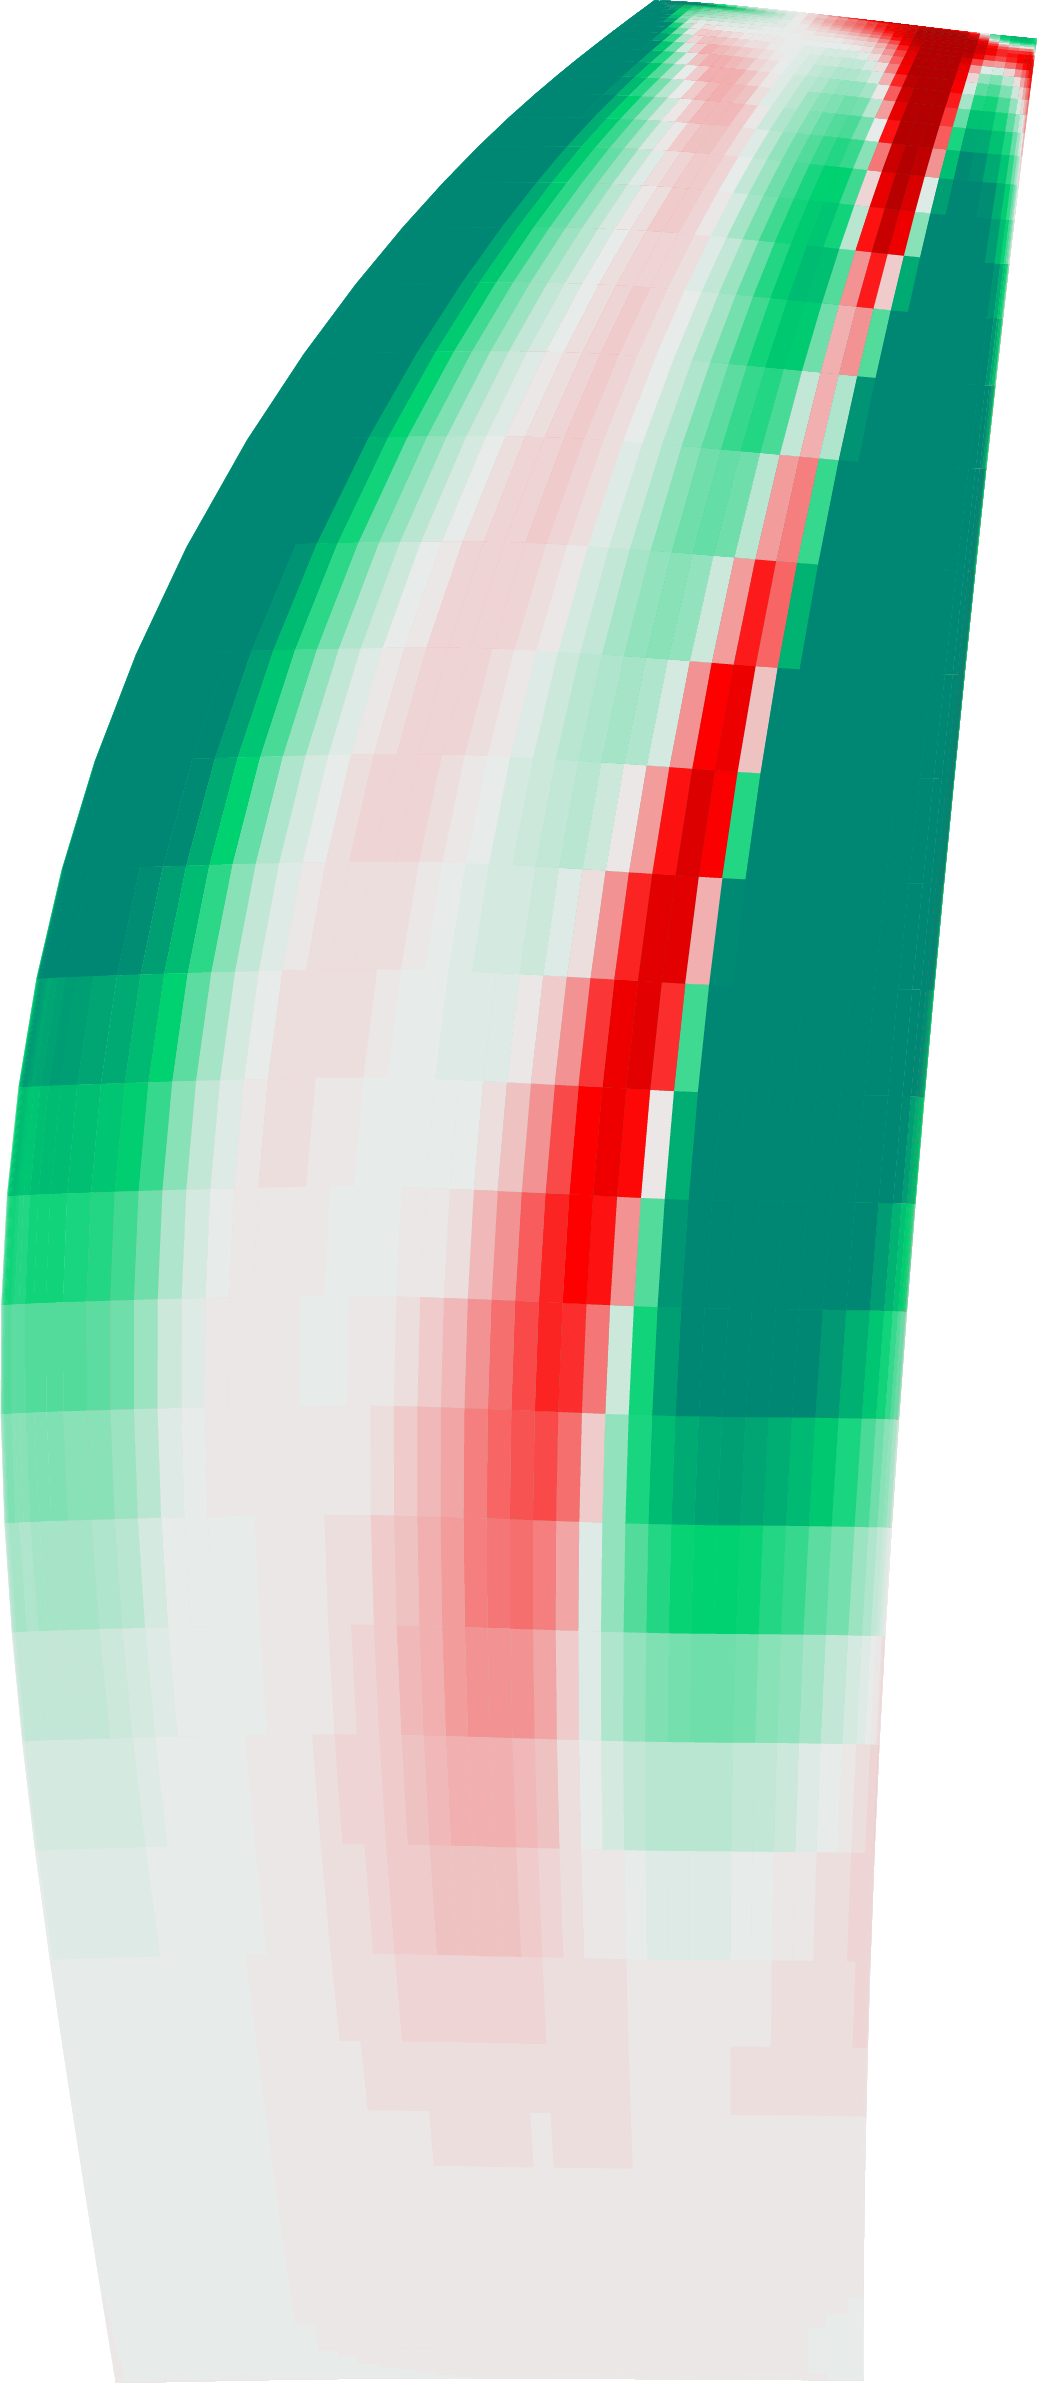
\includegraphics[width=0.12\textwidth]{DREAM_HS_HBT_N5_AEL_H1M1TD3_roe3_sa_local_damping_SS.png}
   & 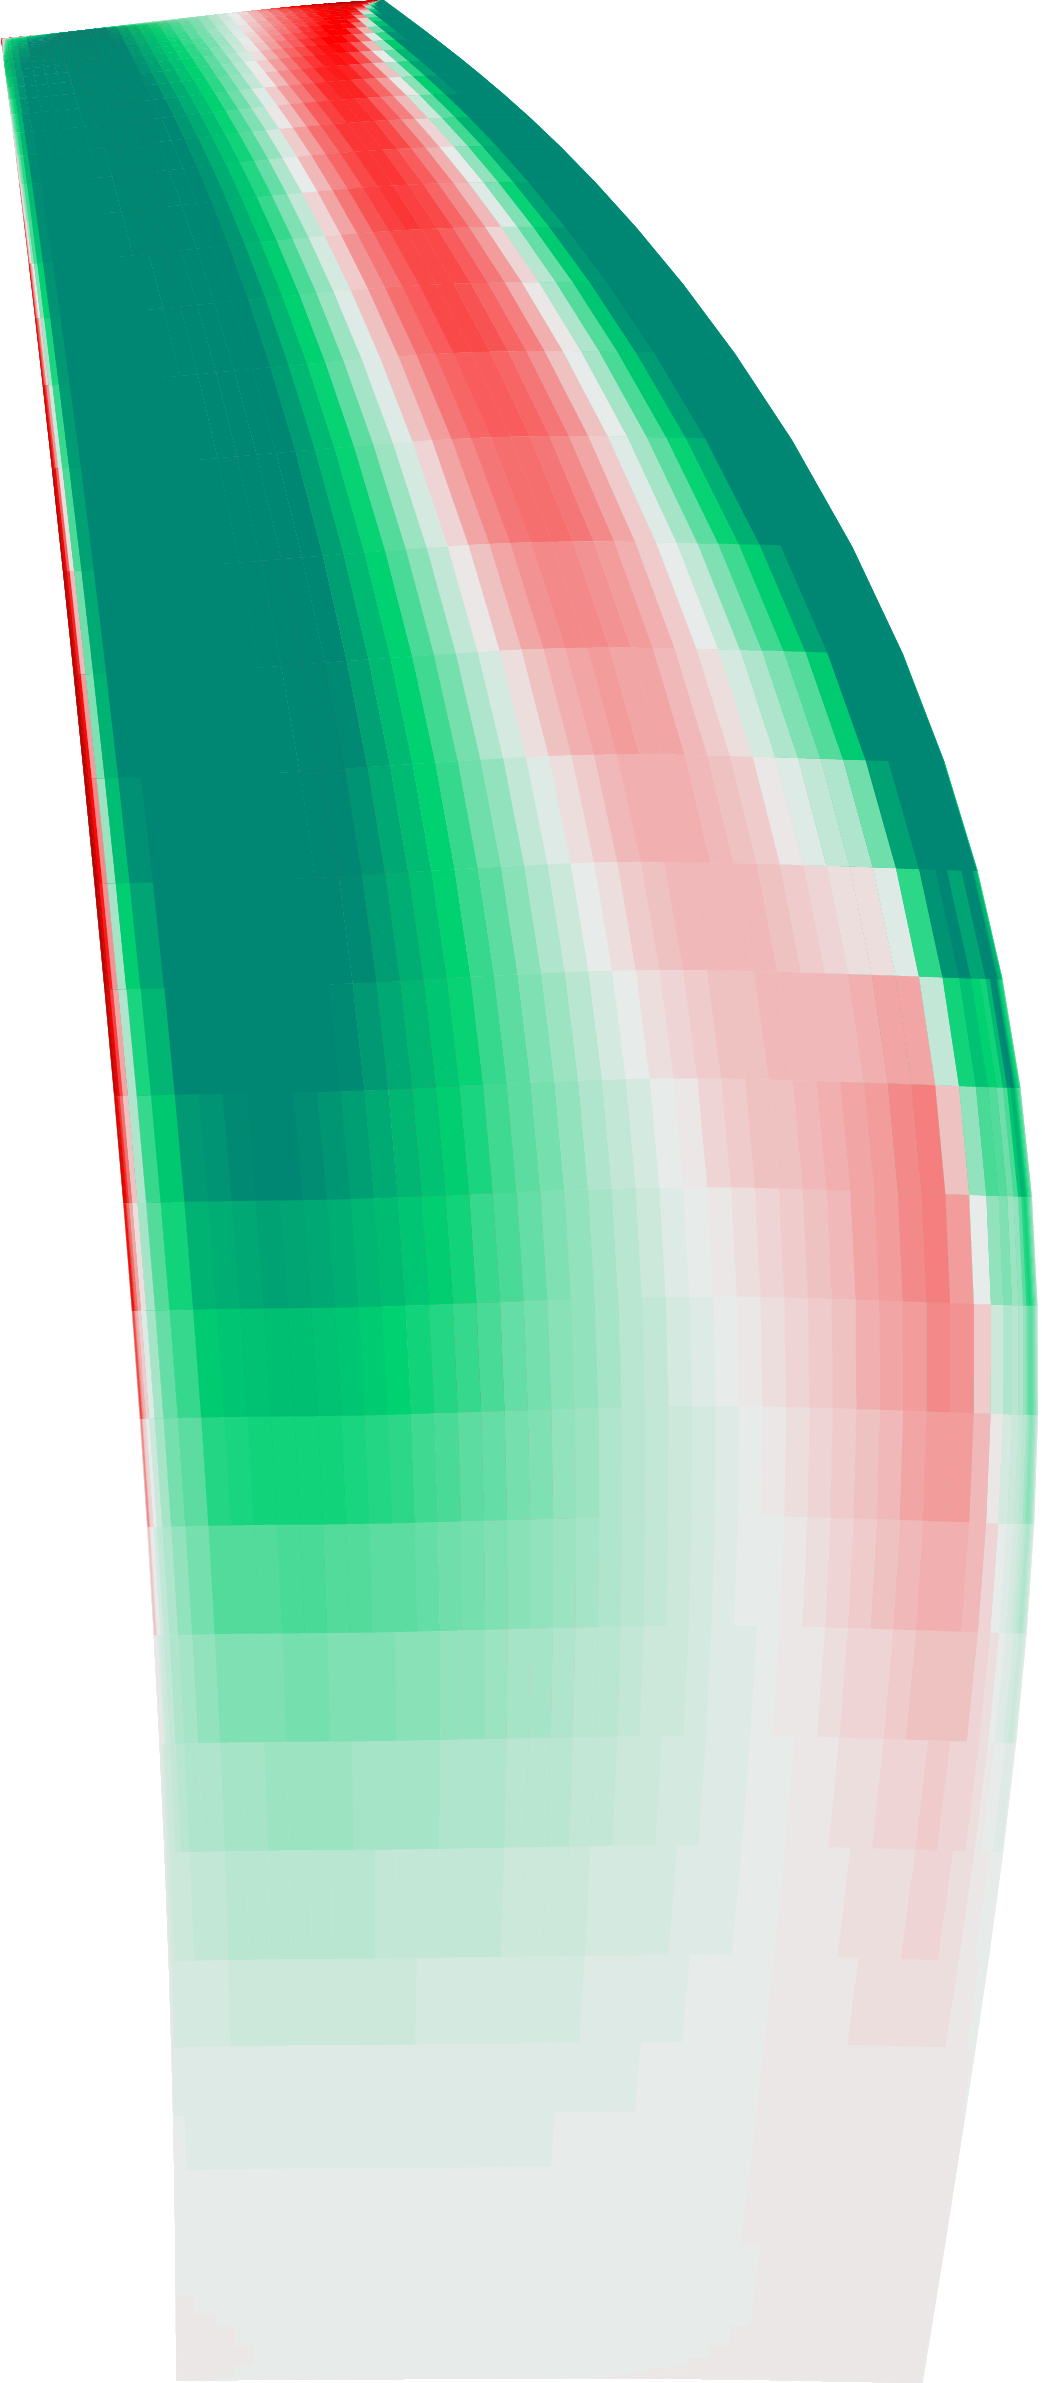
\includegraphics[width=0.12\textwidth]{DREAM_HS_HBT_N5_AEL_H1M1TD3_roe3_sa_local_damping_PS.png} \\
   & suction side & pressure side & suction side & pressure side \\
   \bottomrule
 \end{tabular}
 \caption{High-speed isolated configuration: local excitation for modes 2F and 1T.}
 \label{fig:dream_hs_ael_local_damping}
\end{figure}

Firstly, the level of local excitation is larger for the
1T mode than it is for the 2F mode. This is one explication
for the difference in damping amplitude observed above.
This can be attributed again to the displacement related to the
1T mode. In fact, this mode has the tendency to change the
local angle of attack of the blade, yielding an unadapted
inflow velocity. This angle of attack drives, for the most part,
the aerodynamic behavior around the blade. Therefore, a small
change in angle of attack can have a strong impact on the loading and
the local excitation might be emphasized.
Compared to the low-speed configuration, the local excitation
is always positive on the leading edge of the blade, meaning
that the change in angle of attack and in dihedral angle
produces for the torsional and the flection mode, respectively,
is a positive feature for the damping.

Secondly, the influence of the IBPA remains limited for the
two modes. The global phenomenology is
kept unchanged even though the amplitude varies.
For the torsional mode, the local excitation of
the tip of the blade seems to be sensitive 
to the IBPA. This is the tip vortex region, and
advanced post-processing procedures might be required
to fully understand the behavior of local excitation
near the tip of the blades.

Globally the shape of the local excitation contours
is much more complicated on the high-speed configuration
compared to the low-speed one. In fact, 
not only the modes inflection lines become inflection lines
for the local excitation, but also the shock and 
the flow that develops in the tip region are important.

\subsection{Influence of the number of harmonics on the aeroelastic results}
\label{sub:dream_hs_convergence_ael}

To assess the convergence of the capture of the damping by the multi-frequential
HB approach, four set of frequencies are studied to
run the HB computations on the second flection mode
of the high-speed CROR configuration. For each computation, the 
vibration frequency is considered with one to several harmonics
of the blade passing frequency of the rear rotor. As indicated in
Sec.~\ref{par:choice_of_frequencies}, several approaches exist to
truncate the frequency sets. Here, only the "cross grid" truncation 
pattern is used with only one aeroelastic frequency.
\begin{figure}[htp]
 \ra{1.3} \centering
 \begin{tabular}{r|cccc}
   \toprule
   & \multicolumn{4}{c}{
        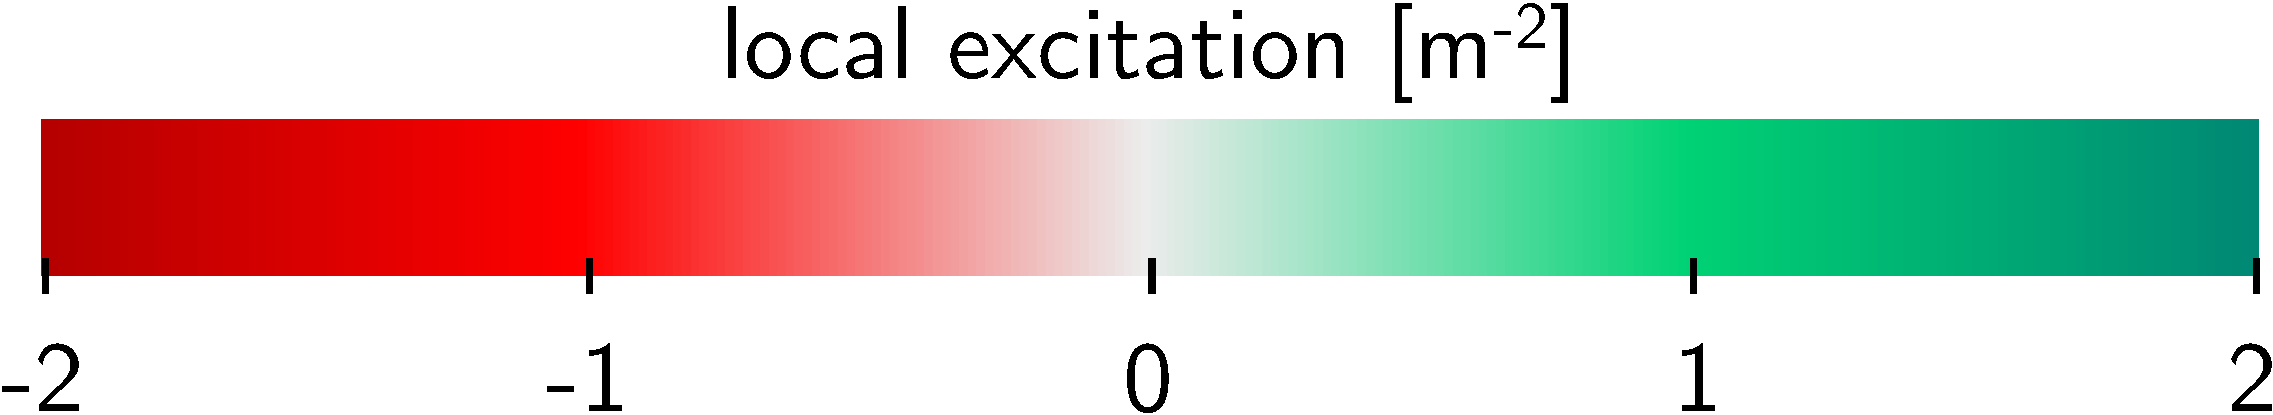
\includegraphics[width=0.22\textwidth]{dream_hs_damping_scale.pdf}} \\
   & $N=2$ & $N=3$ & $N=4$ & $N=5$ \\
   \midrule
   \rotatebox{90}{\quad\quad\quad suction side} 
   & 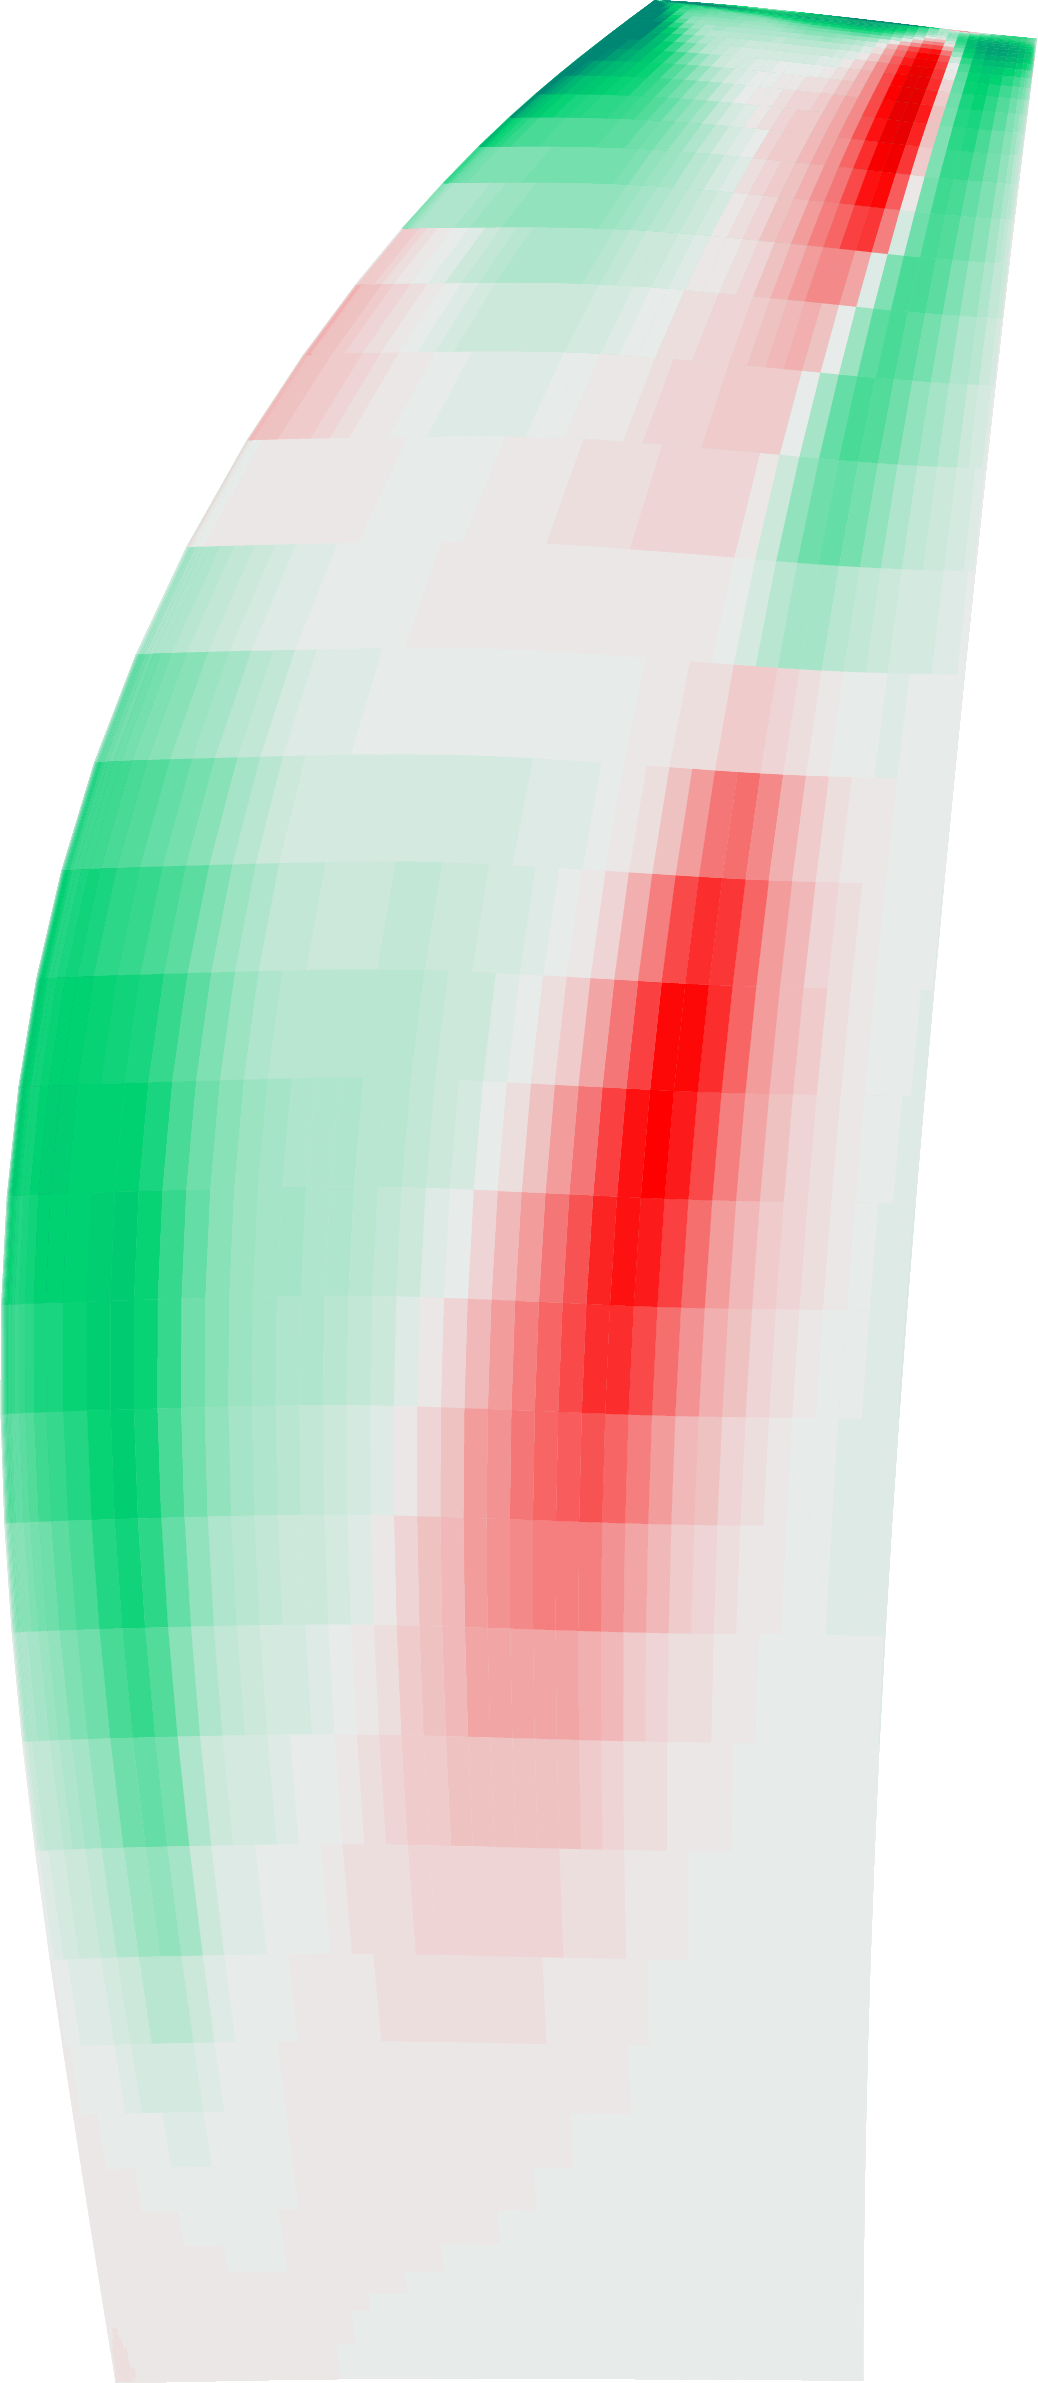
\includegraphics[width=0.12\textwidth]{DREAM_HS_HBT_N2_AEL_H1M2FD-1_roe3_sa_local_damping_SS.png}
   & 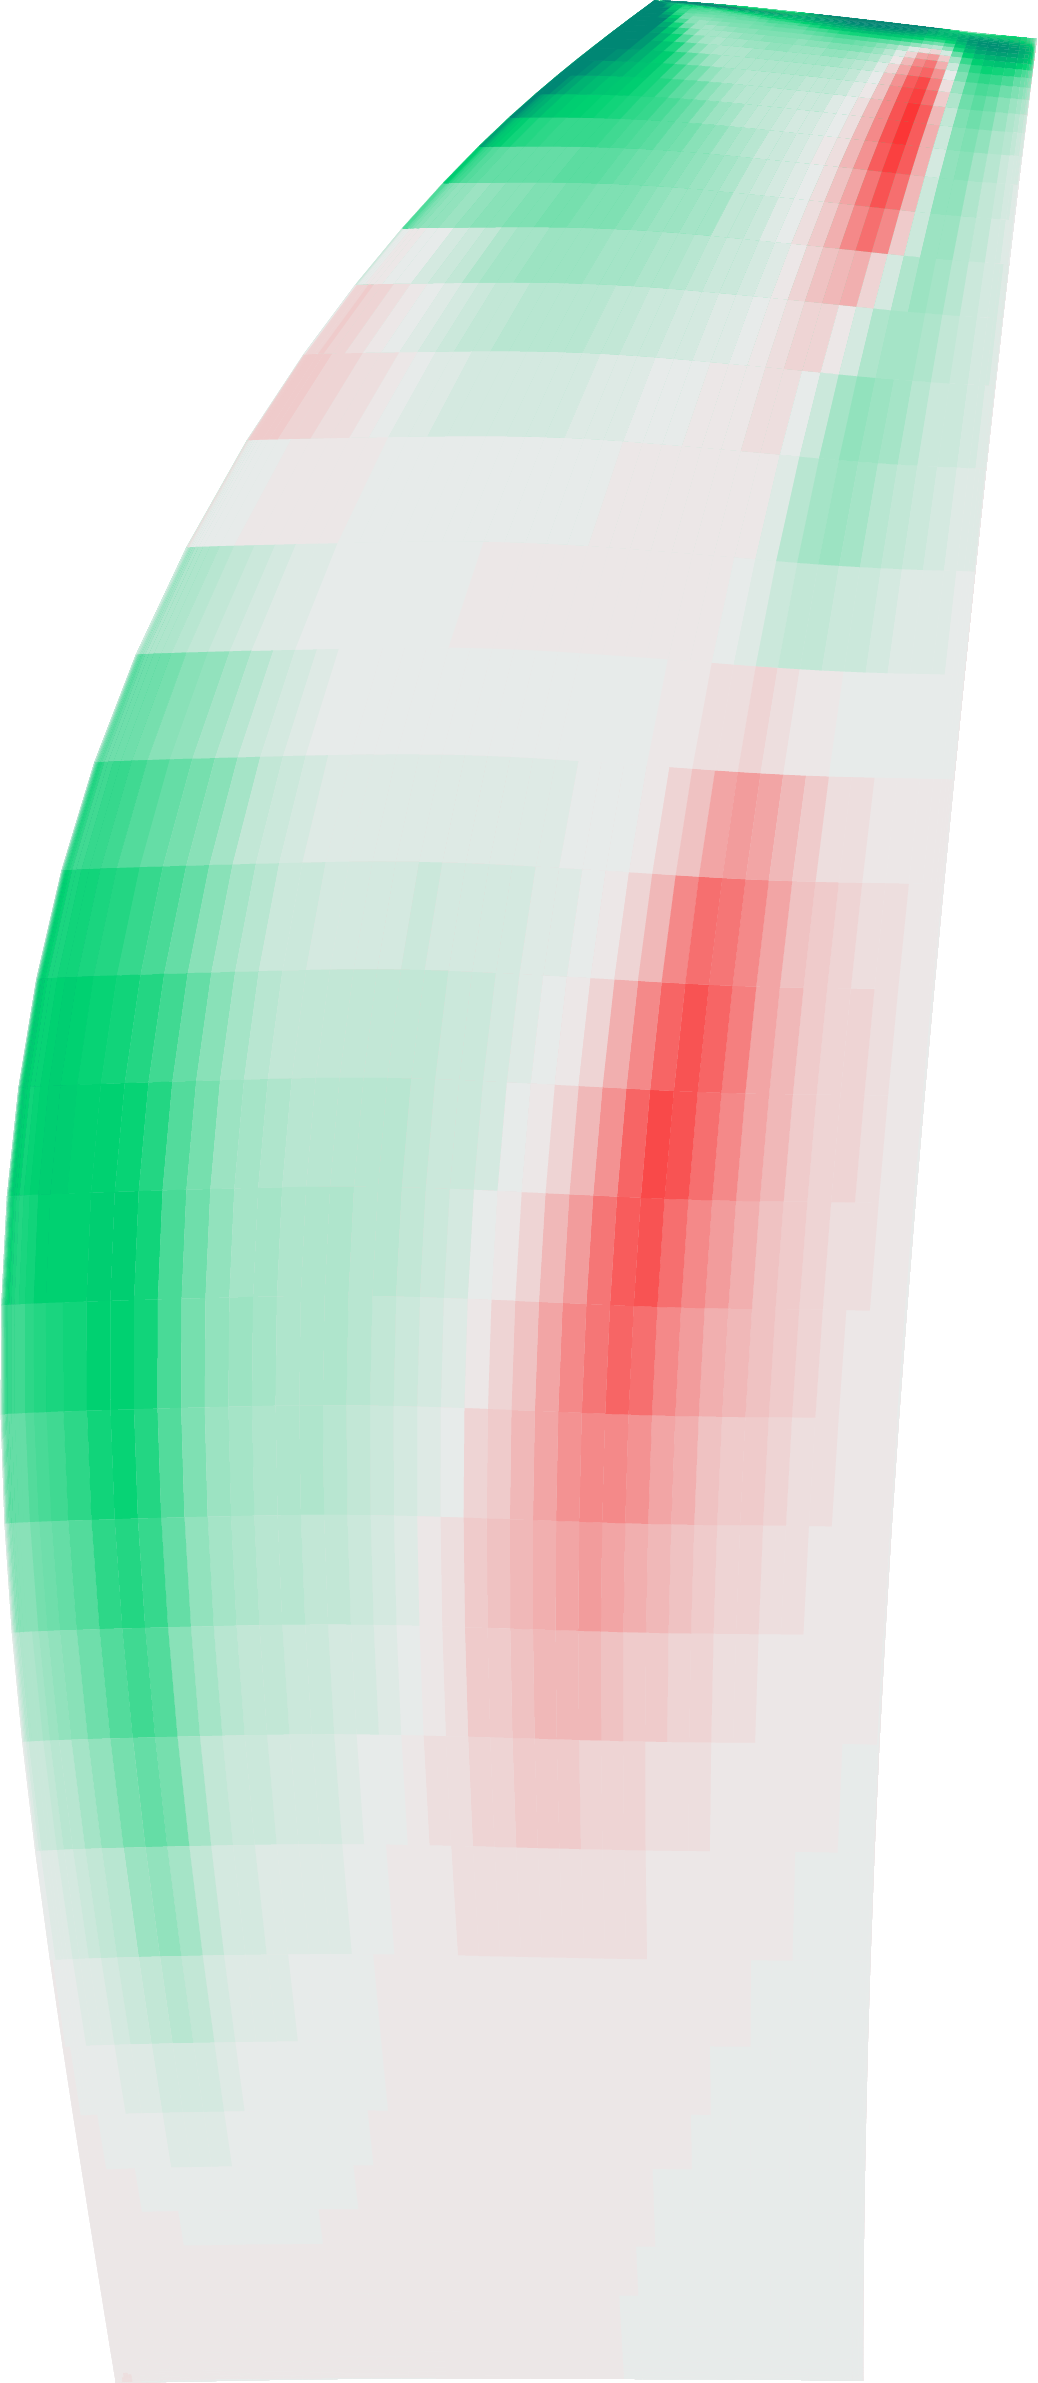
\includegraphics[width=0.12\textwidth]{DREAM_HS_HBT_N3_AEL_H1M2FD-1_roe3_sa_local_damping_SS.png}
   & 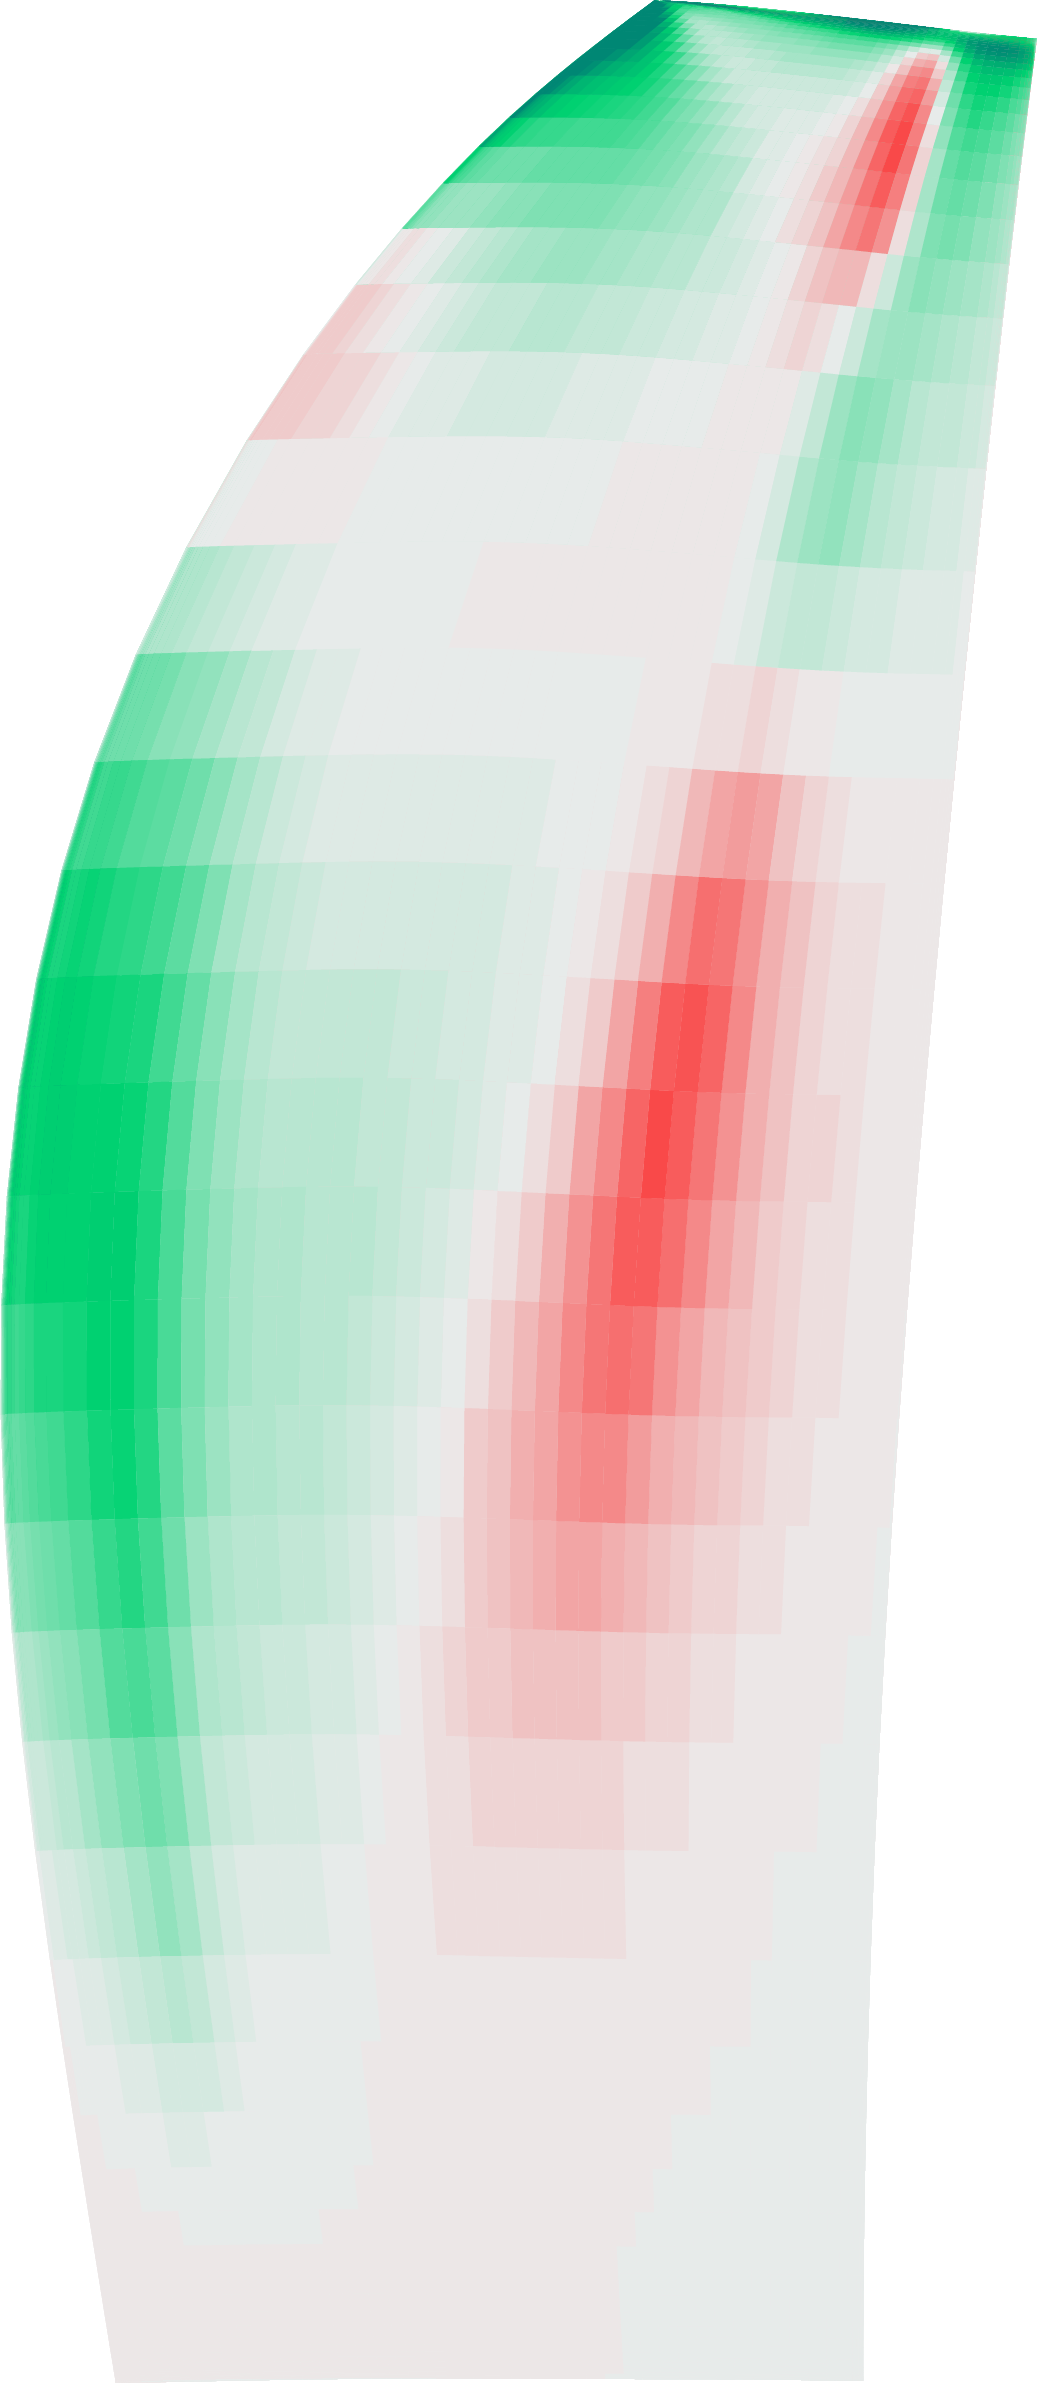
\includegraphics[width=0.12\textwidth]{DREAM_HS_HBT_N4_AEL_H1M2FD-1_roe3_sa_local_damping_SS.png}
   & 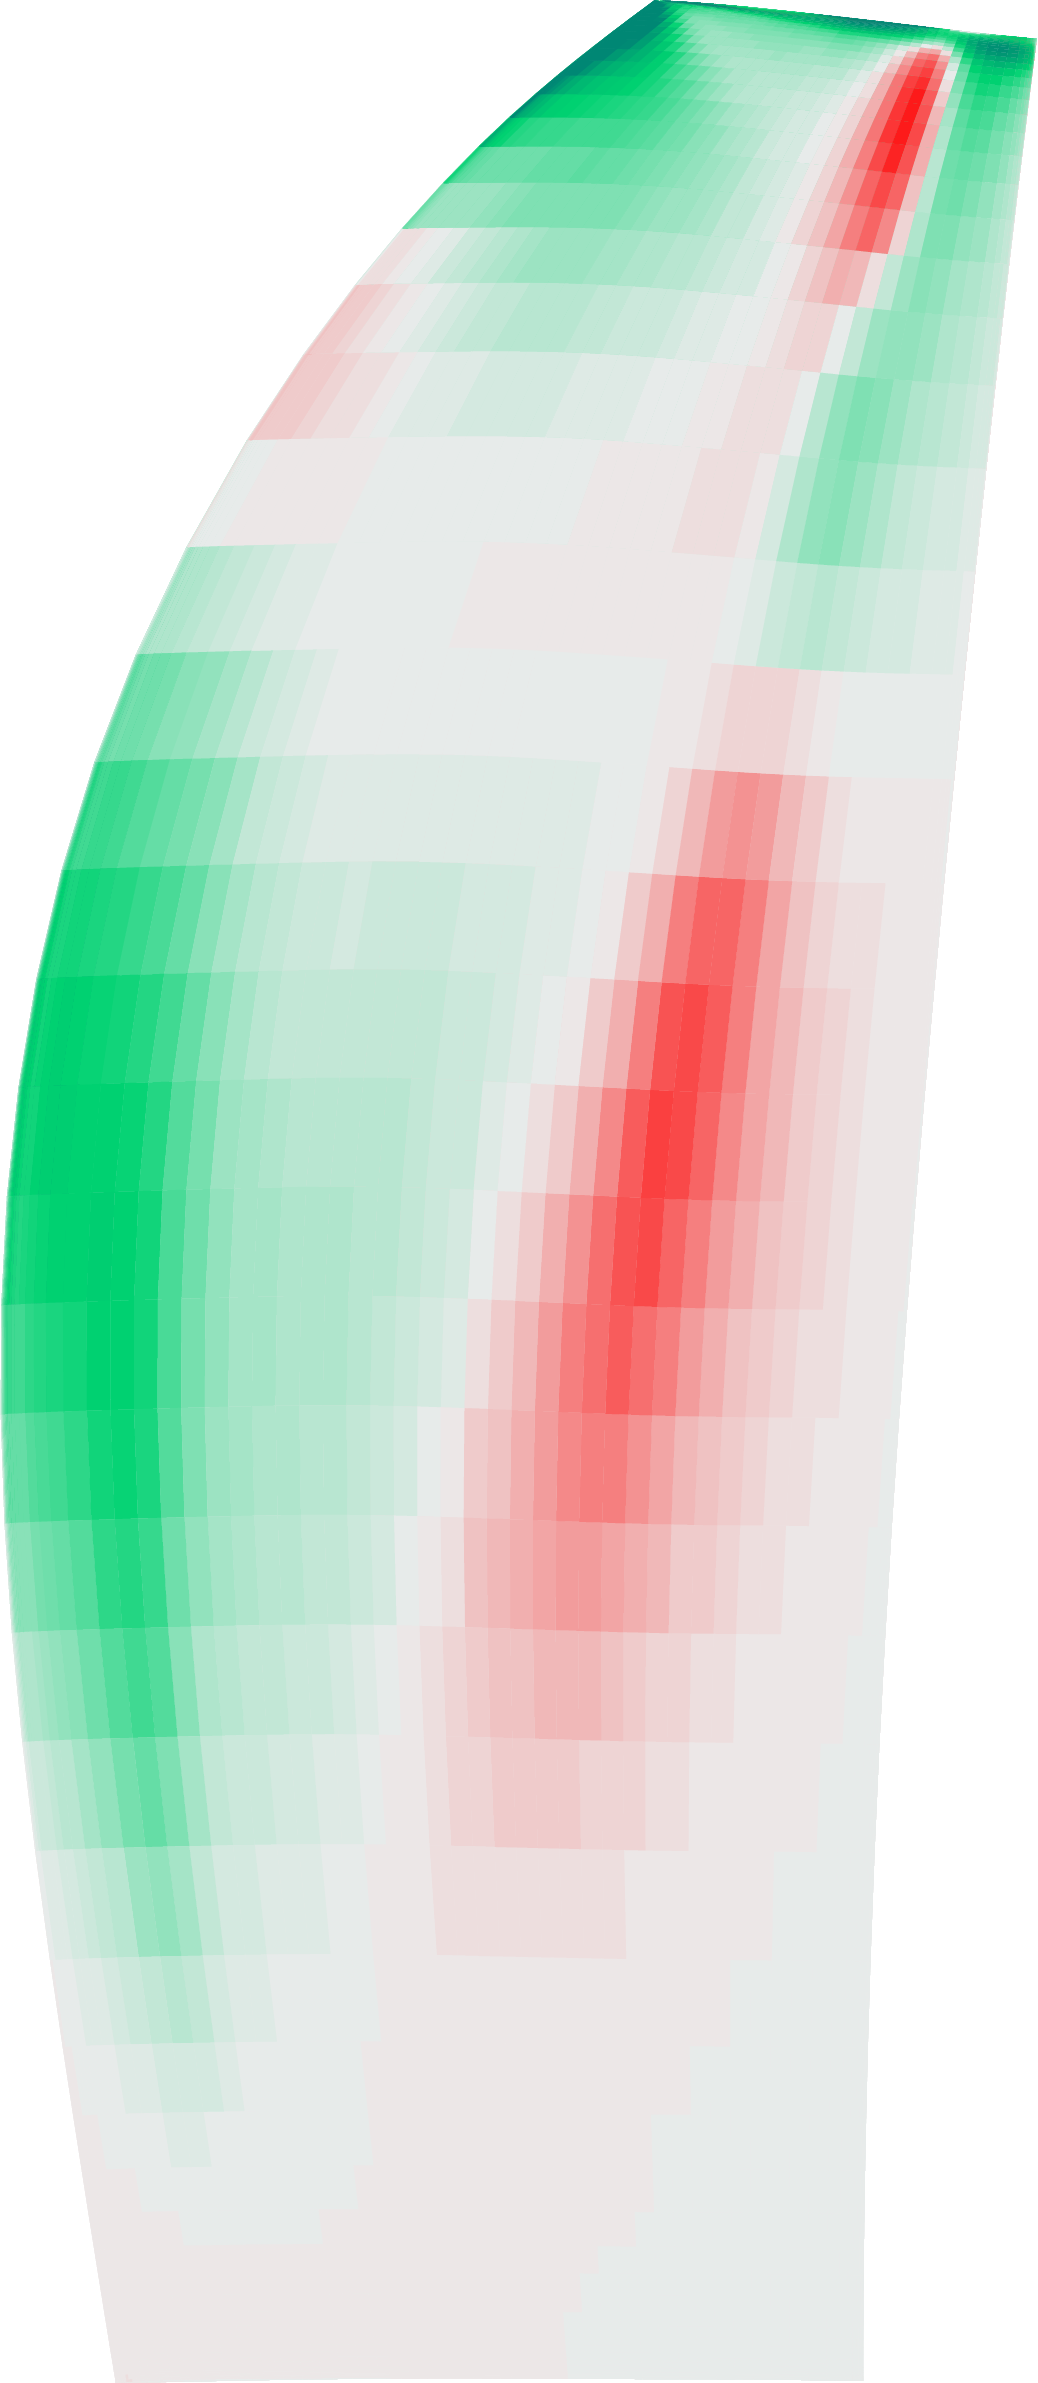
\includegraphics[width=0.12\textwidth]{DREAM_HS_HBT_N5_AEL_H1M2FD-1_roe3_sa_local_damping_SS.png} \\
   \rotatebox{90}{\quad\quad\quad pressure side} 
   & 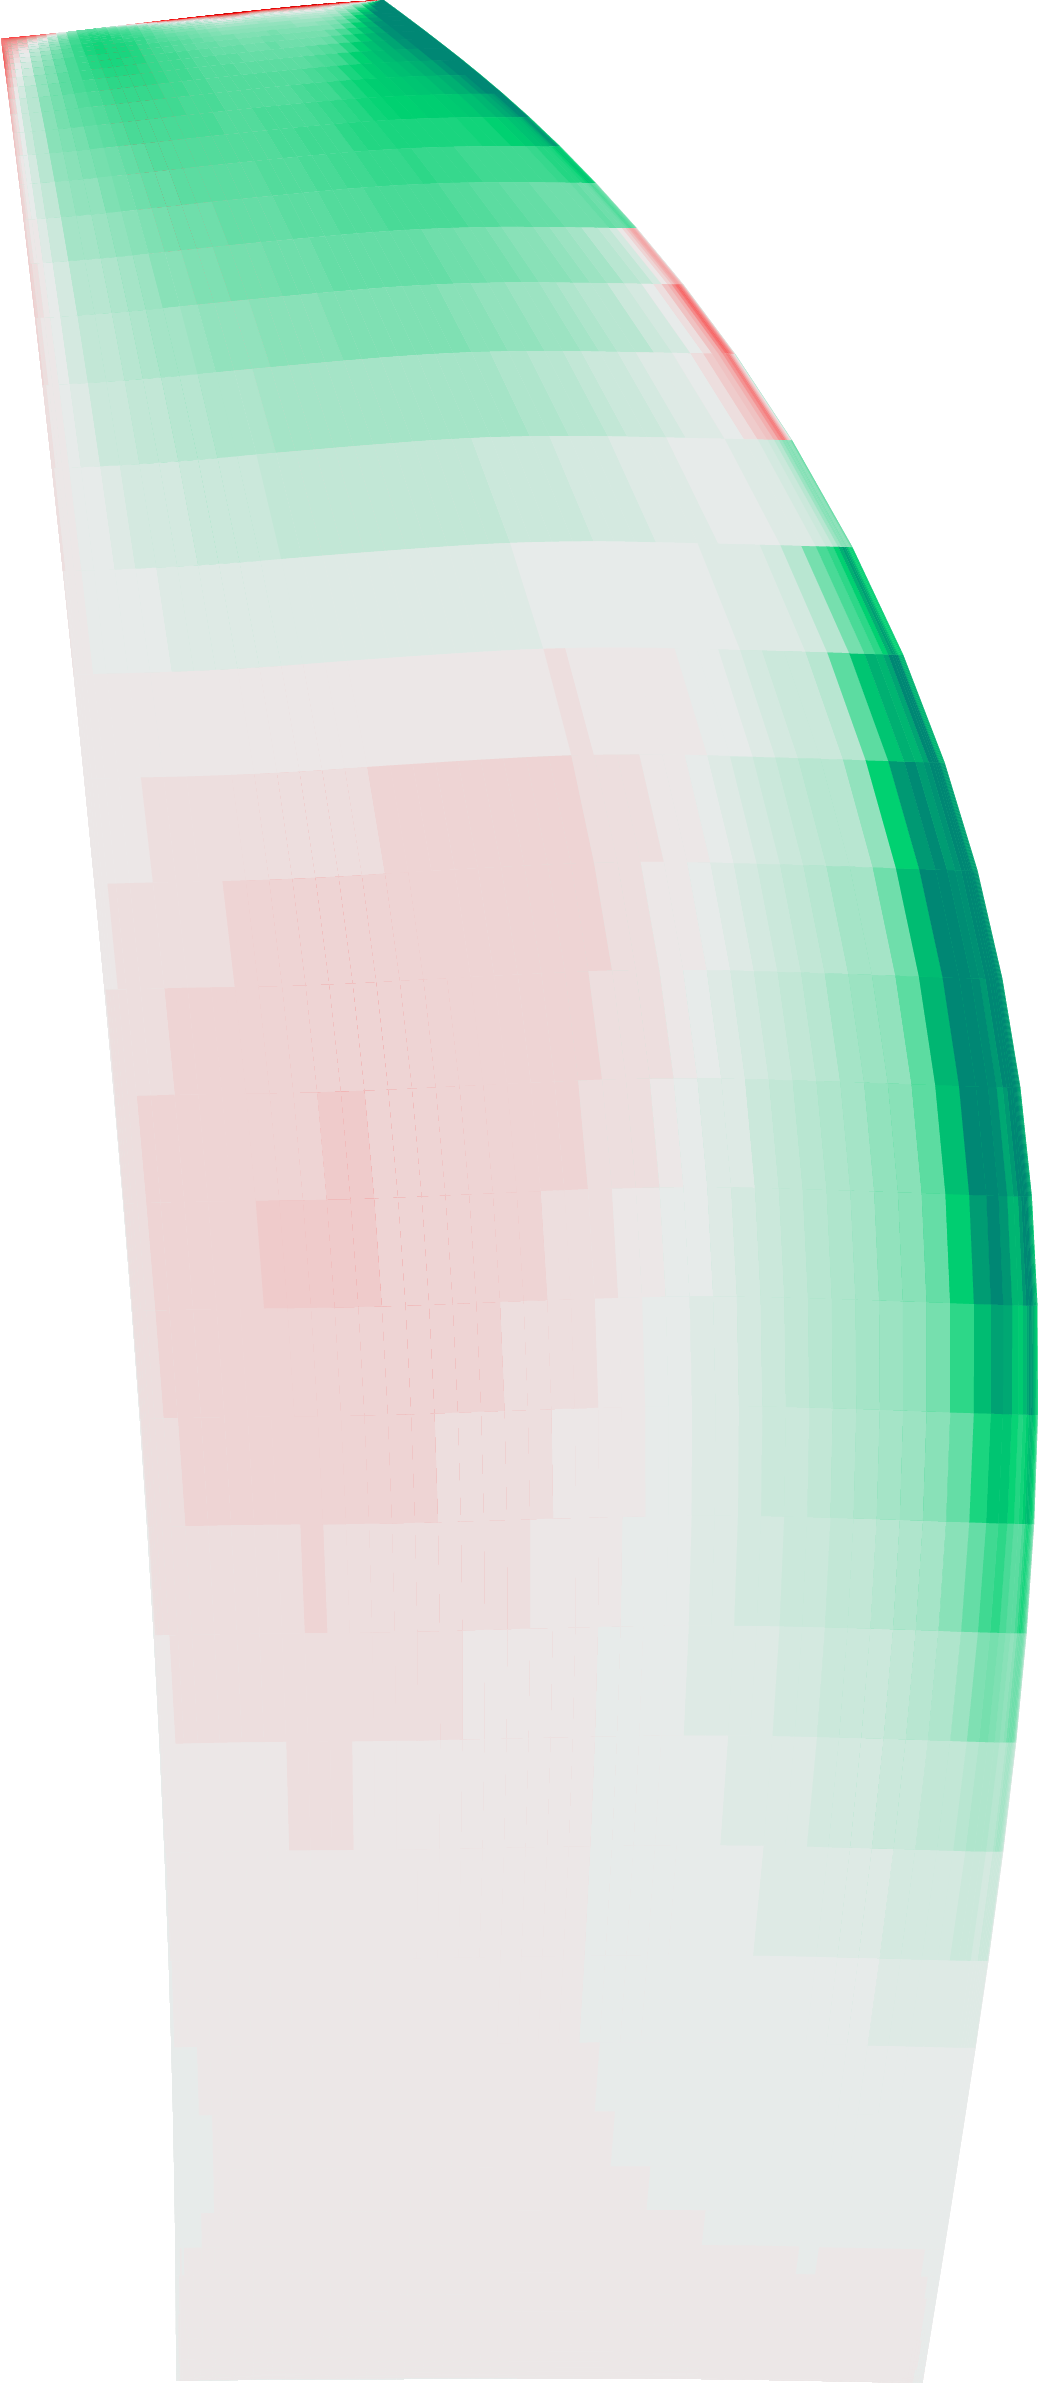
\includegraphics[width=0.12\textwidth]{DREAM_HS_HBT_N2_AEL_H1M2FD-1_roe3_sa_local_damping_PS.png}
   & 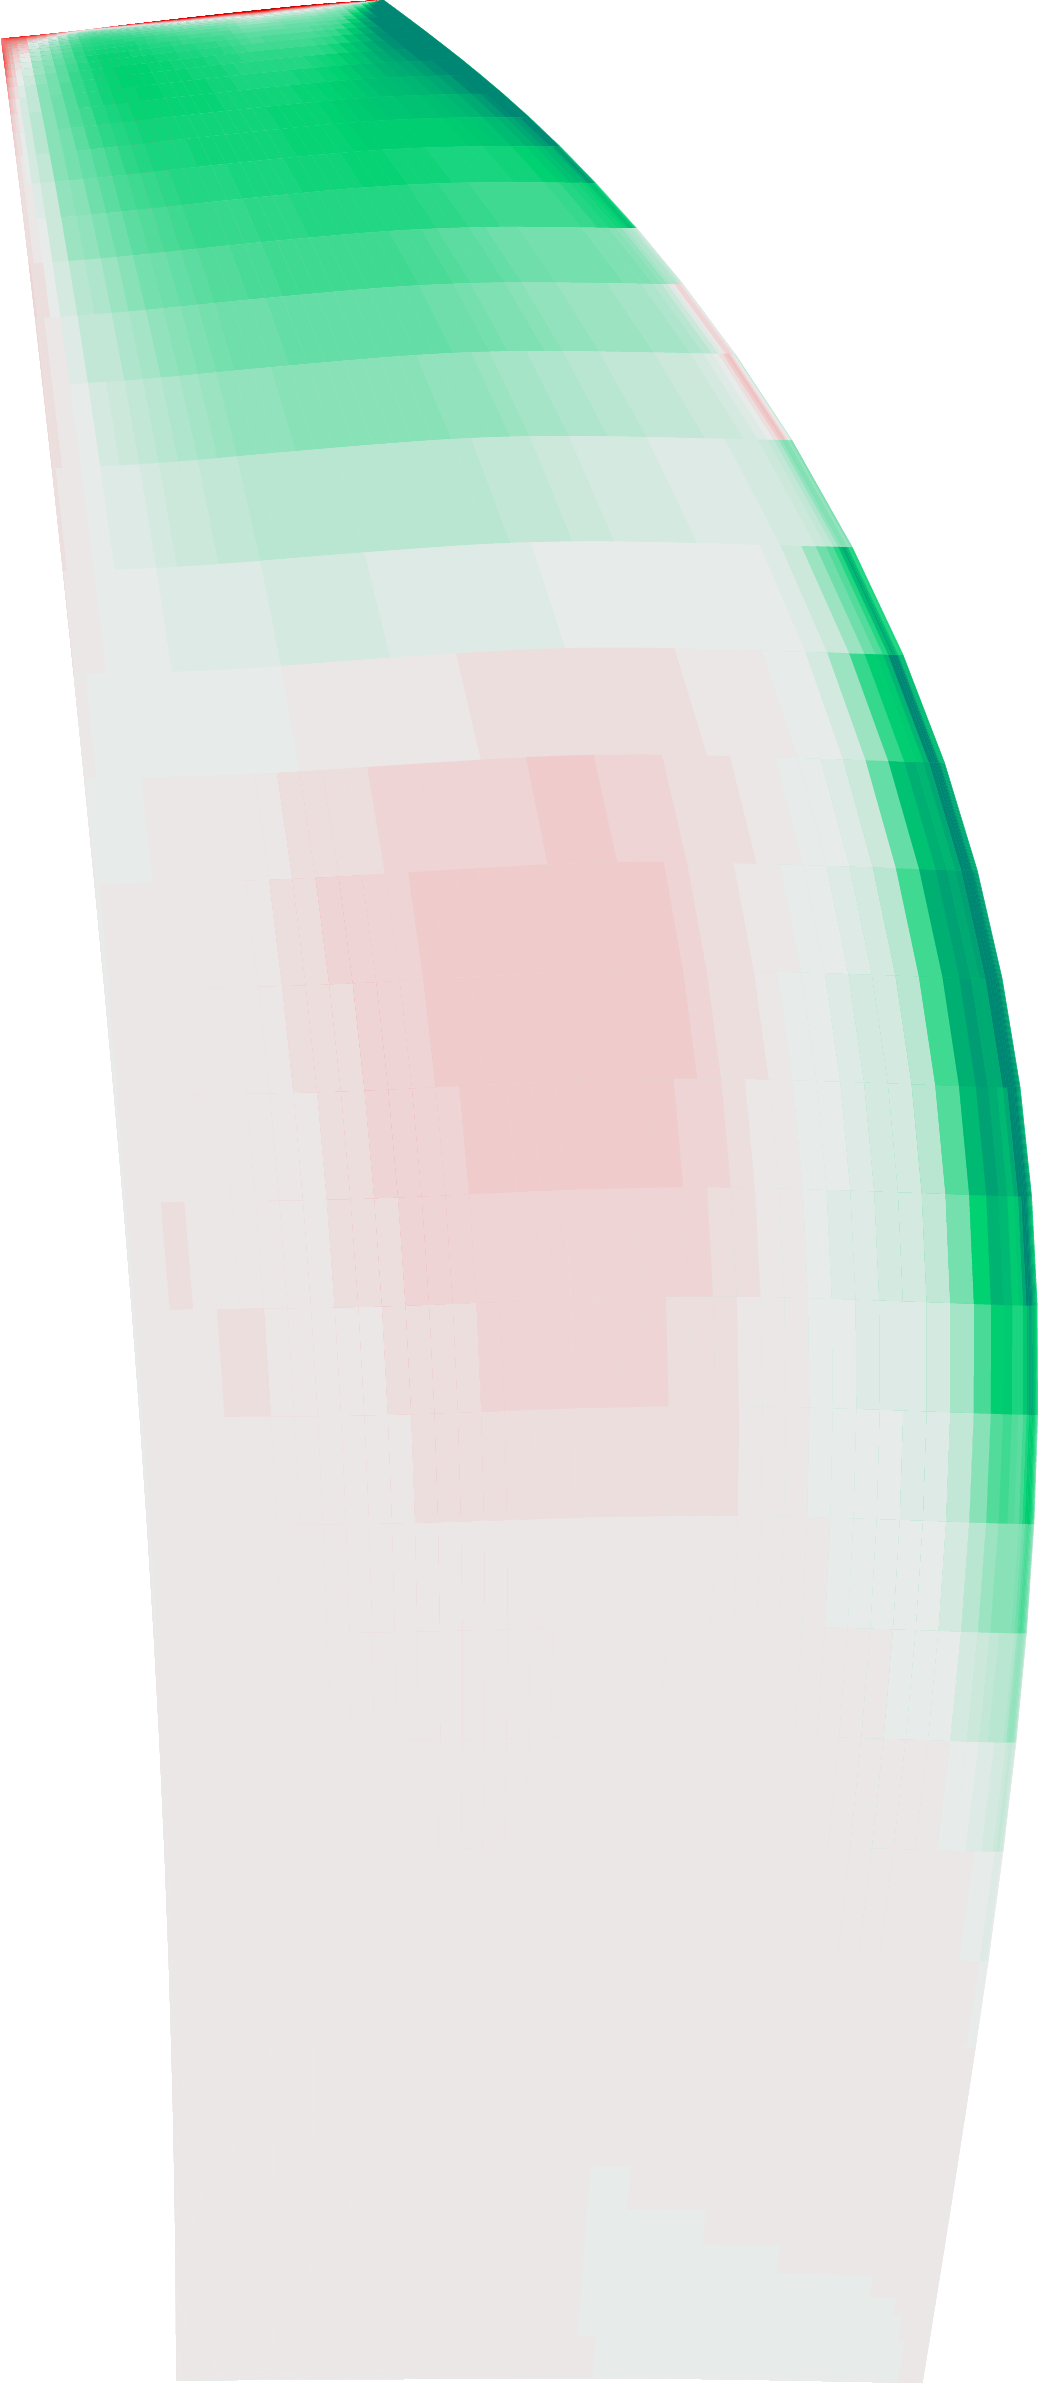
\includegraphics[width=0.12\textwidth]{DREAM_HS_HBT_N3_AEL_H1M2FD-1_roe3_sa_local_damping_PS.png}
   & 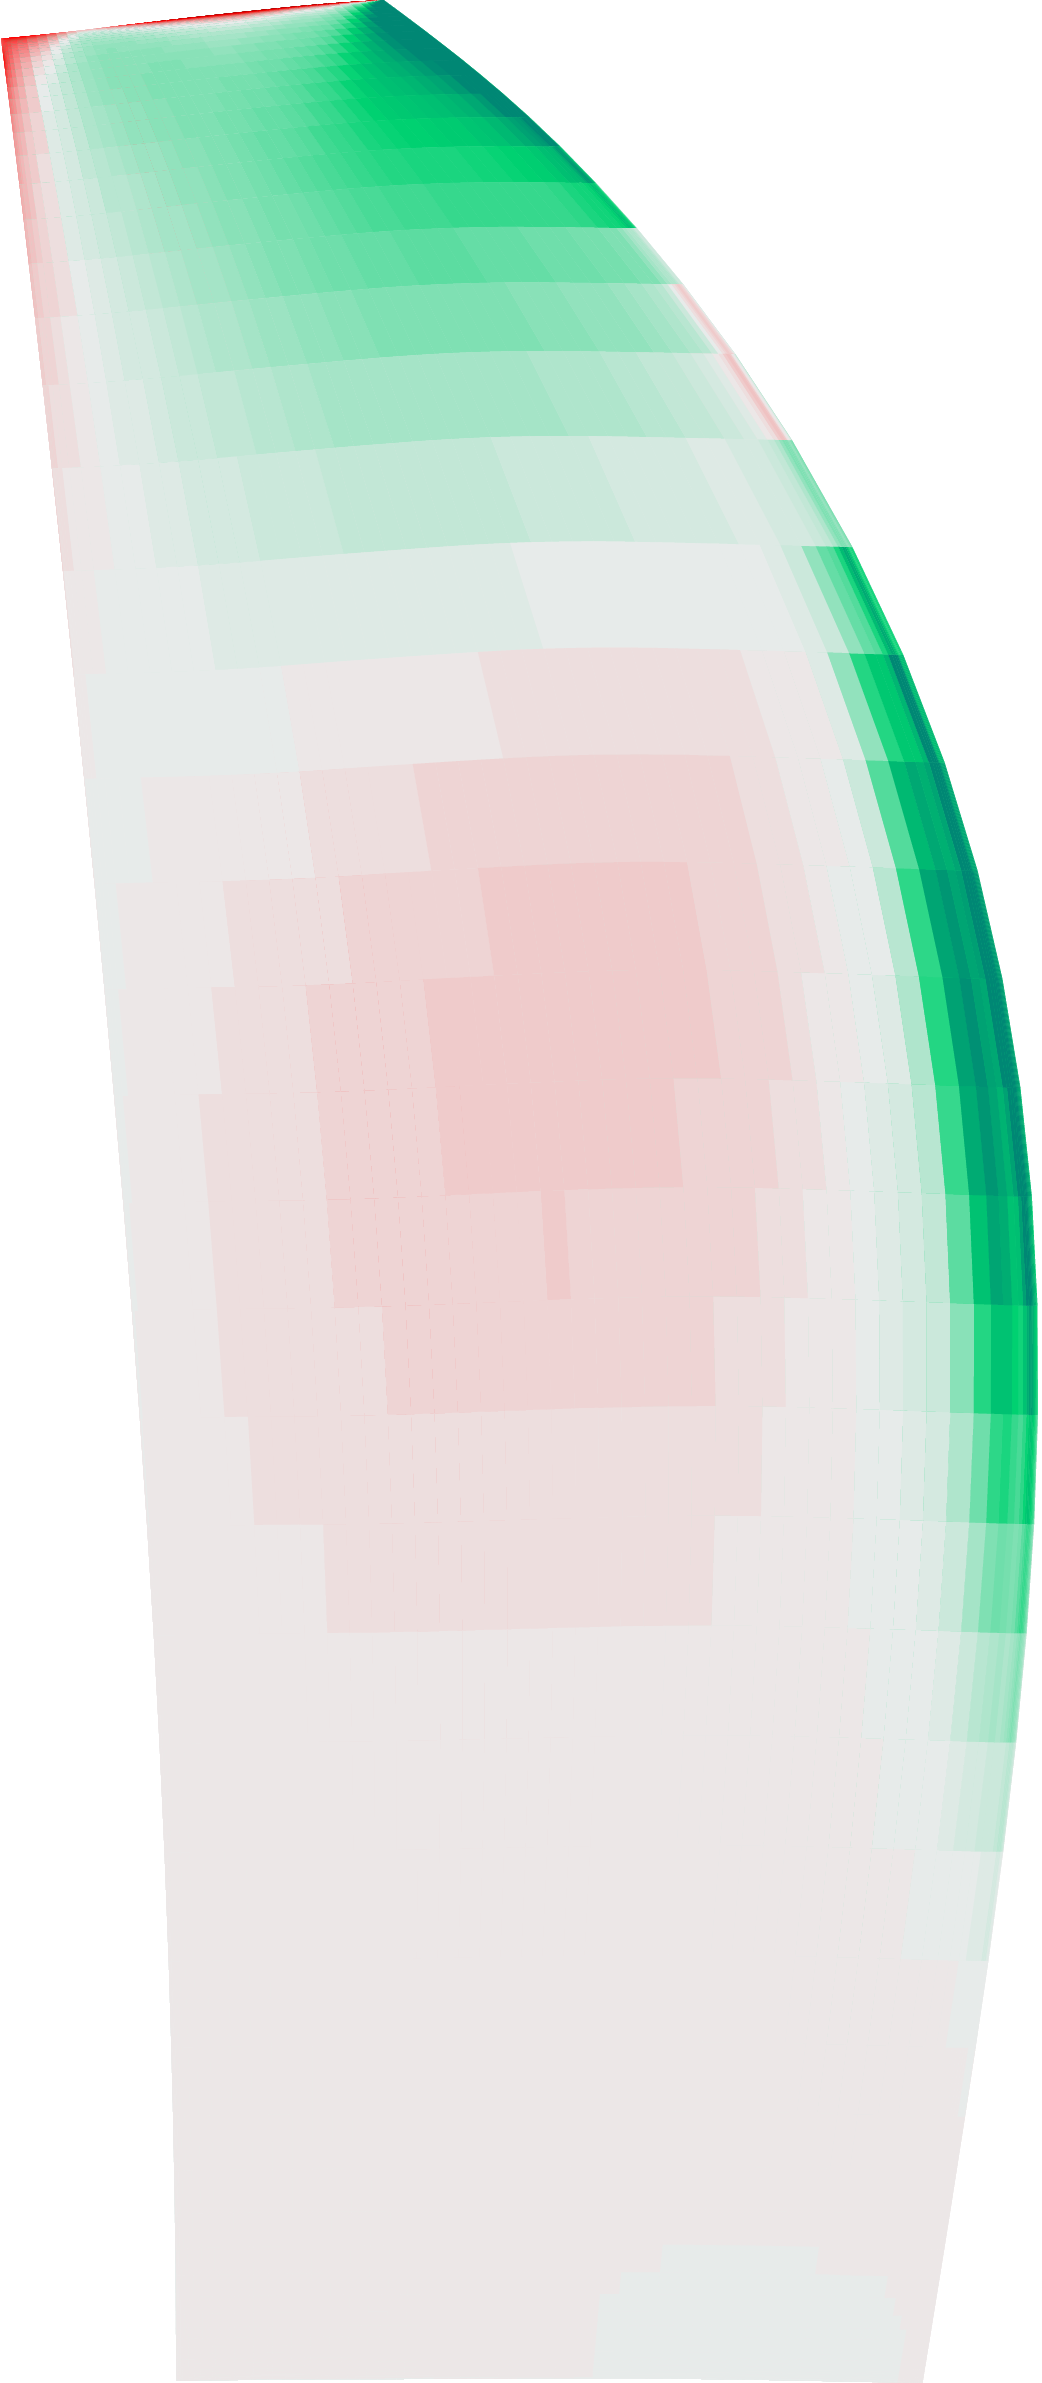
\includegraphics[width=0.12\textwidth]{DREAM_HS_HBT_N4_AEL_H1M2FD-1_roe3_sa_local_damping_PS.png}
   & 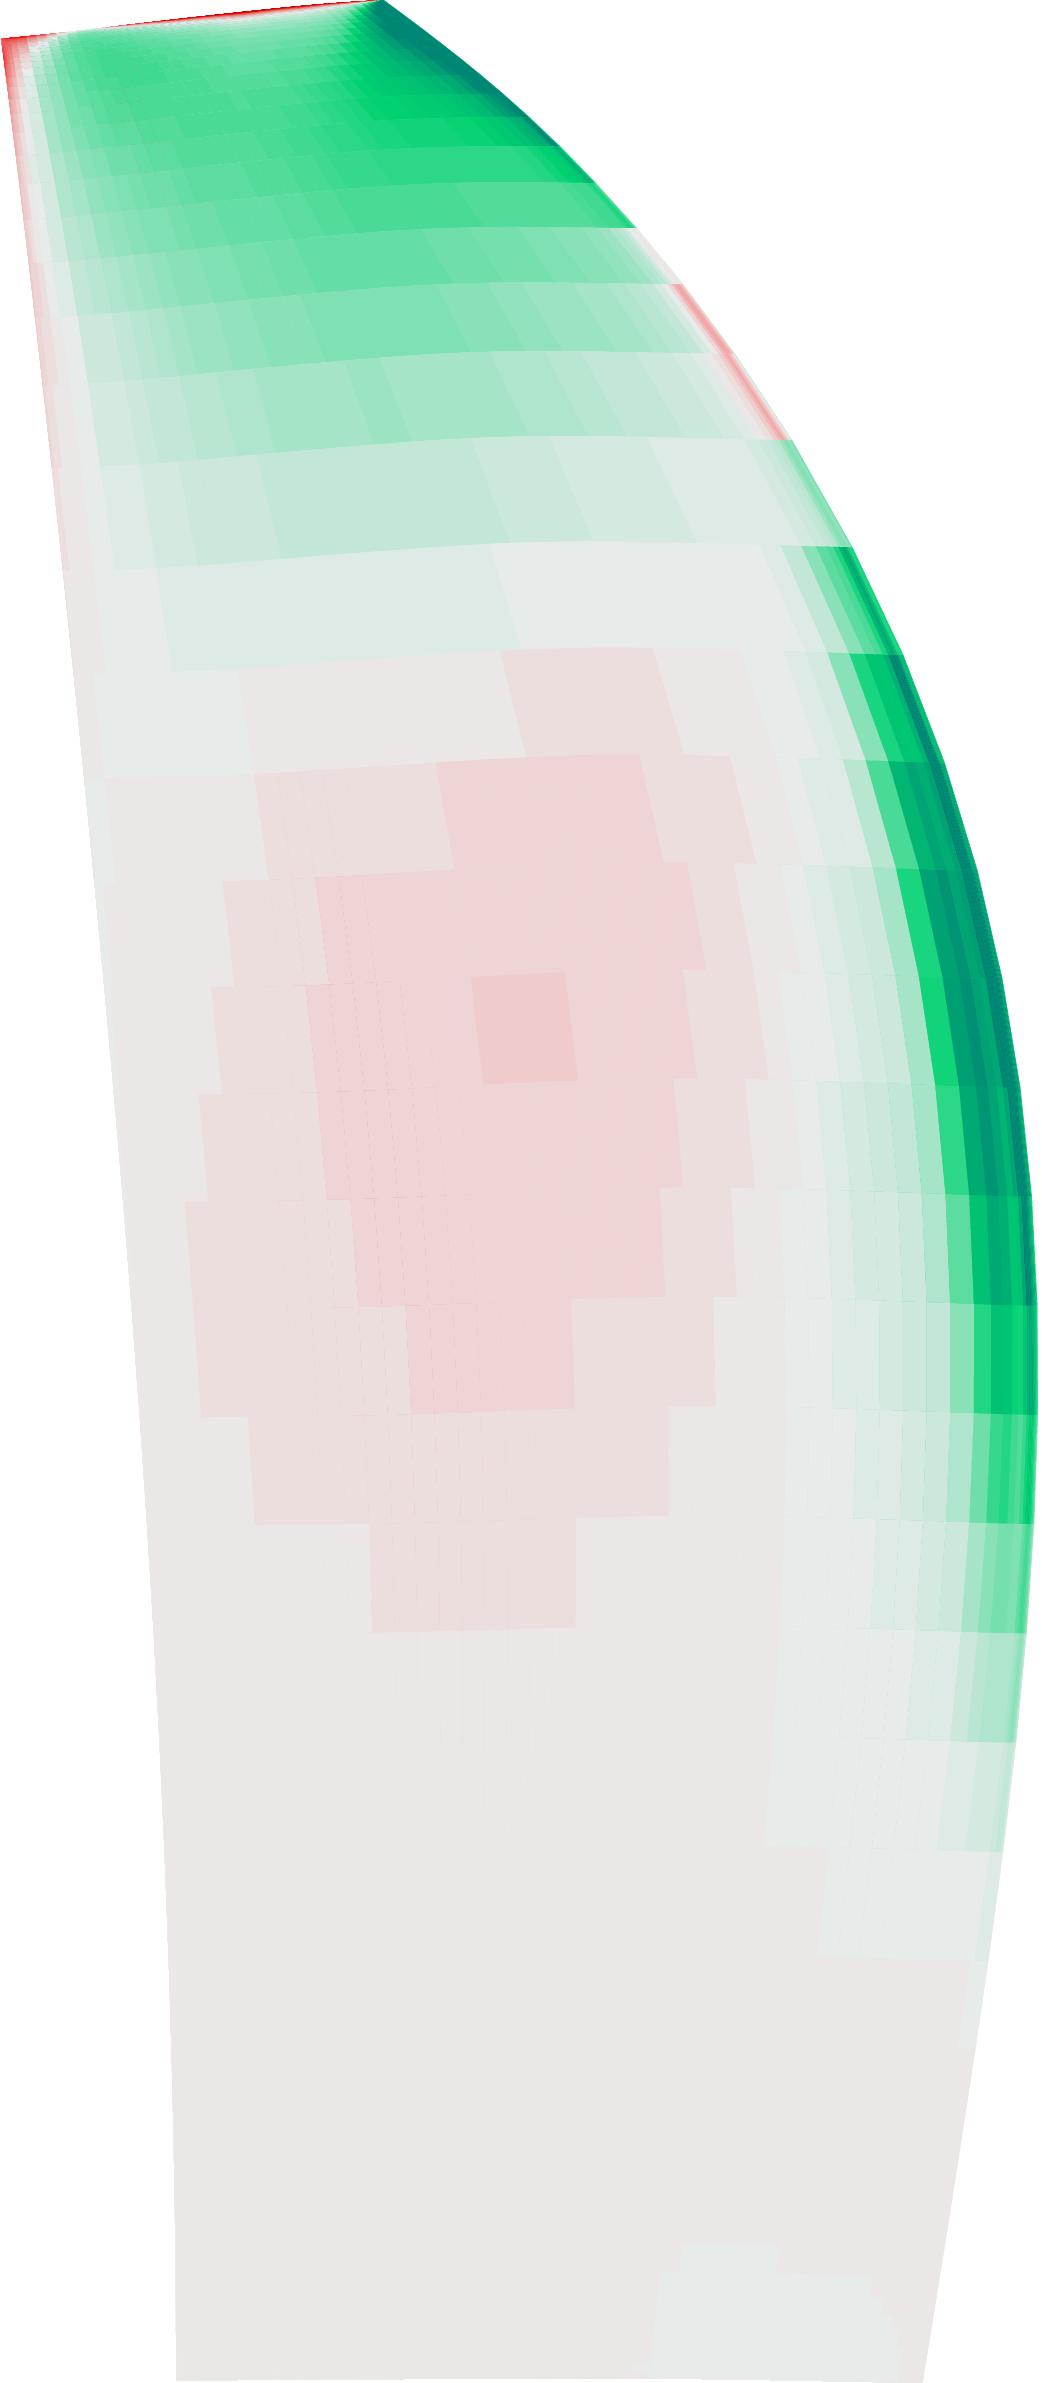
\includegraphics[width=0.12\textwidth]{DREAM_HS_HBT_N5_AEL_H1M2FD-1_roe3_sa_local_damping_PS.png} \\
   \bottomrule
   \multicolumn{1}{c}{}& \\
   \multicolumn{1}{c}{} & \multicolumn{4}{c}{
        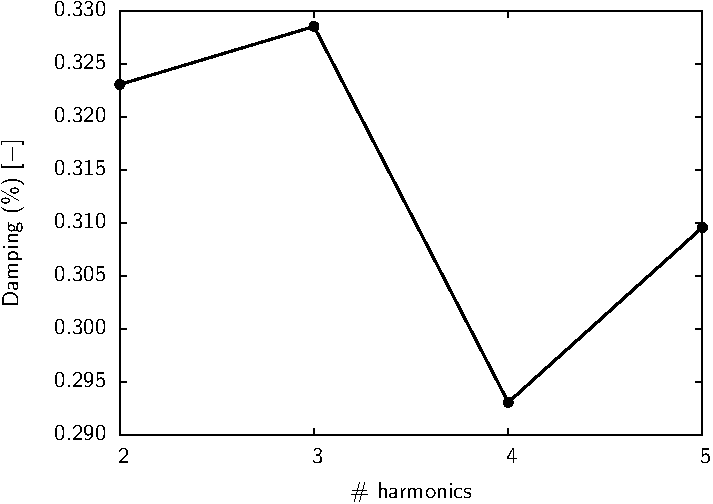
\includegraphics[width=0.45\textwidth]{DREAM_HS_COMVERGENCE_DAMPING.pdf}} \\
 \end{tabular}
 \caption{High-speed isolated configuration: convergence of local excitation and damping.}
 \label{fig:dream_hs_ael_convergence_damping}
\end{figure}
The local excitation and damping results are 
shown in Figure~\ref{fig:dream_hs_ael_convergence_damping}.
Raising the number of harmonics of the rear rotor blade passing frequency
changes the damping by at-most 10\% but the contours
of the local excitation are kept nearly unchanged. Only small differences
are observed, that integrated produces the 10\%
observed on the damping value. Further investigation of the
convergence for the choice of frequencies are needed, but
this has not been done on this work.
